\documentclass[11pt,a4paper]{article}

\usepackage[utf8]{inputenc}
\usepackage[T1]{fontenc}
\usepackage{lmodern}
\usepackage[margin=1.9cm]{geometry}
\usepackage{amsmath}
\usepackage{booktabs}
\usepackage{array}
\usepackage{tabularx}
\usepackage{longtable}
\usepackage{graphicx}
\usepackage{xcolor}
\usepackage{hyperref}
\usepackage{microtype}
\usepackage{caption}
\usepackage{float}
\usepackage{fancyhdr}
\usepackage{enumitem}

\definecolor{navy}{HTML}{102A43}
\definecolor{blue}{HTML}{1677B8}
\definecolor{green}{HTML}{2A9D6F}
\definecolor{light}{HTML}{F4F7FA}
\definecolor{muted}{HTML}{627D98}
\hypersetup{
  colorlinks=true,
  linkcolor=blue,
  citecolor=blue,
  urlcolor=blue,
  pdftitle={Professional Preprocessing and Chronological Model Evaluation for Paris Apartment Valuation},
  pdfauthor={Badr Ettousy}
}
\graphicspath{{../../visuals/model_evaluation/}{../../visuals/phase3/}{../../visuals/phase2/}}
\captionsetup{font=small,labelfont=bf}
\setlength{\parskip}{0.38em}
\setlength{\parindent}{0pt}
\renewcommand{\arraystretch}{1.15}
\pagestyle{fancy}
\fancyhf{}
\fancyhead[L]{\small\textcolor{muted}{Paris AVM --- preprocessing and model evaluation}}
\fancyhead[R]{\small\textcolor{muted}{Badr Ettousy}}
\fancyfoot[C]{\thepage}
\setlength{\headheight}{14pt}

\newcommand{\metriccard}[2]{%
  \colorbox{light}{\begin{minipage}[c][1.55cm][c]{0.215\textwidth}
  \centering\textcolor{navy}{\Large\textbf{#1}}\\[-0.1em]
  \small\textcolor{muted}{#2}
  \end{minipage}}}

\title{\textcolor{navy}{\textbf{Professional Data Science Report}}\\[0.25em]
\large Complete Preprocessing, Leakage Controls and\\
Chronological Model Evaluation for Paris Apartment Valuation}
\author{Badr Ettousy}
\date{August 2026}

\begin{document}
\maketitle

\begin{abstract}
This report documents the complete preprocessing and empirical evaluation of a
Paris apartment automated valuation model (AVM). The fixed analytical cohort
contains 143,009 ordinary apartment sales from 2021--2025. Five feature layers
are implemented: property characteristics, transaction time, spatial identity,
strictly historical comparable sales, and external building/energy/neighborhood
enrichment. The resulting Phase 2 table has 60 columns and a 44-input model
contract; the enriched Phase 3 table has 141 columns and a 100-input selected
model contract. Historical comparable features use only transactions at least
90 days old. DPE records are accepted only when their diagnostic date is no
later than the sale date. Model development uses 2021--2023, configuration
selection uses 2024, and 28,330 transactions from 2025 form the untouched final
test cohort. The selected CatBoost model reaches EUR 93,197 mean absolute error
(MAE), EUR 192,809 root mean squared error, $R^2=0.8679$, and 11.70\% median
absolute percentage error. It reduces MAE by EUR 3,231 (3.35\%) relative to the
frozen Phase 2 comparable correction; the paired 95\% bootstrap interval is EUR
2,685--3,730. The gain is positive in every month and arrondissement, but
calibration diagnostics show overprediction at the cheapest decile and
underprediction at the most expensive decile. The model is therefore a strong
automated indication, not a substitute for a certified appraisal.
\end{abstract}

\vspace{0.5em}
\begin{center}
\metriccard{143,009}{audited sales} \hfill
\metriccard{100}{selected inputs} \hfill
\metriccard{EUR 93,197}{2025 MAE} \hfill
\metriccard{3.35\%}{MAE reduction}
\end{center}

\tableofcontents
\clearpage

\section{Executive assessment}

The complete preprocessing and retraining workflow succeeds technically and
empirically. The Gold transaction identity is unchanged across feature layers:
143,009 unique mutations enter Phase 2, and exactly the same ordered mutations
leave Phase 3. All 89 repository tests and 101 artifact subtests pass after
retraining, including dedicated model-evaluation and report-contract checks.

The main result is statistically consistent but deliberately described as
incremental. Phase 3 reduces average absolute error from EUR 96,428 to EUR
93,197 on the same 28,330 sales. The EUR 3,231 paired reduction has a 95\%
bootstrap interval of EUR 2,685--3,730. Accuracy within 20\% increases from
71.69\% to 73.40\%, while $R^2$ increases from 0.8601 to 0.8679. These gains
support the added data engineering; they do not imply causal effects from DPE,
transport or building characteristics.

\begin{figure}[H]
\centering
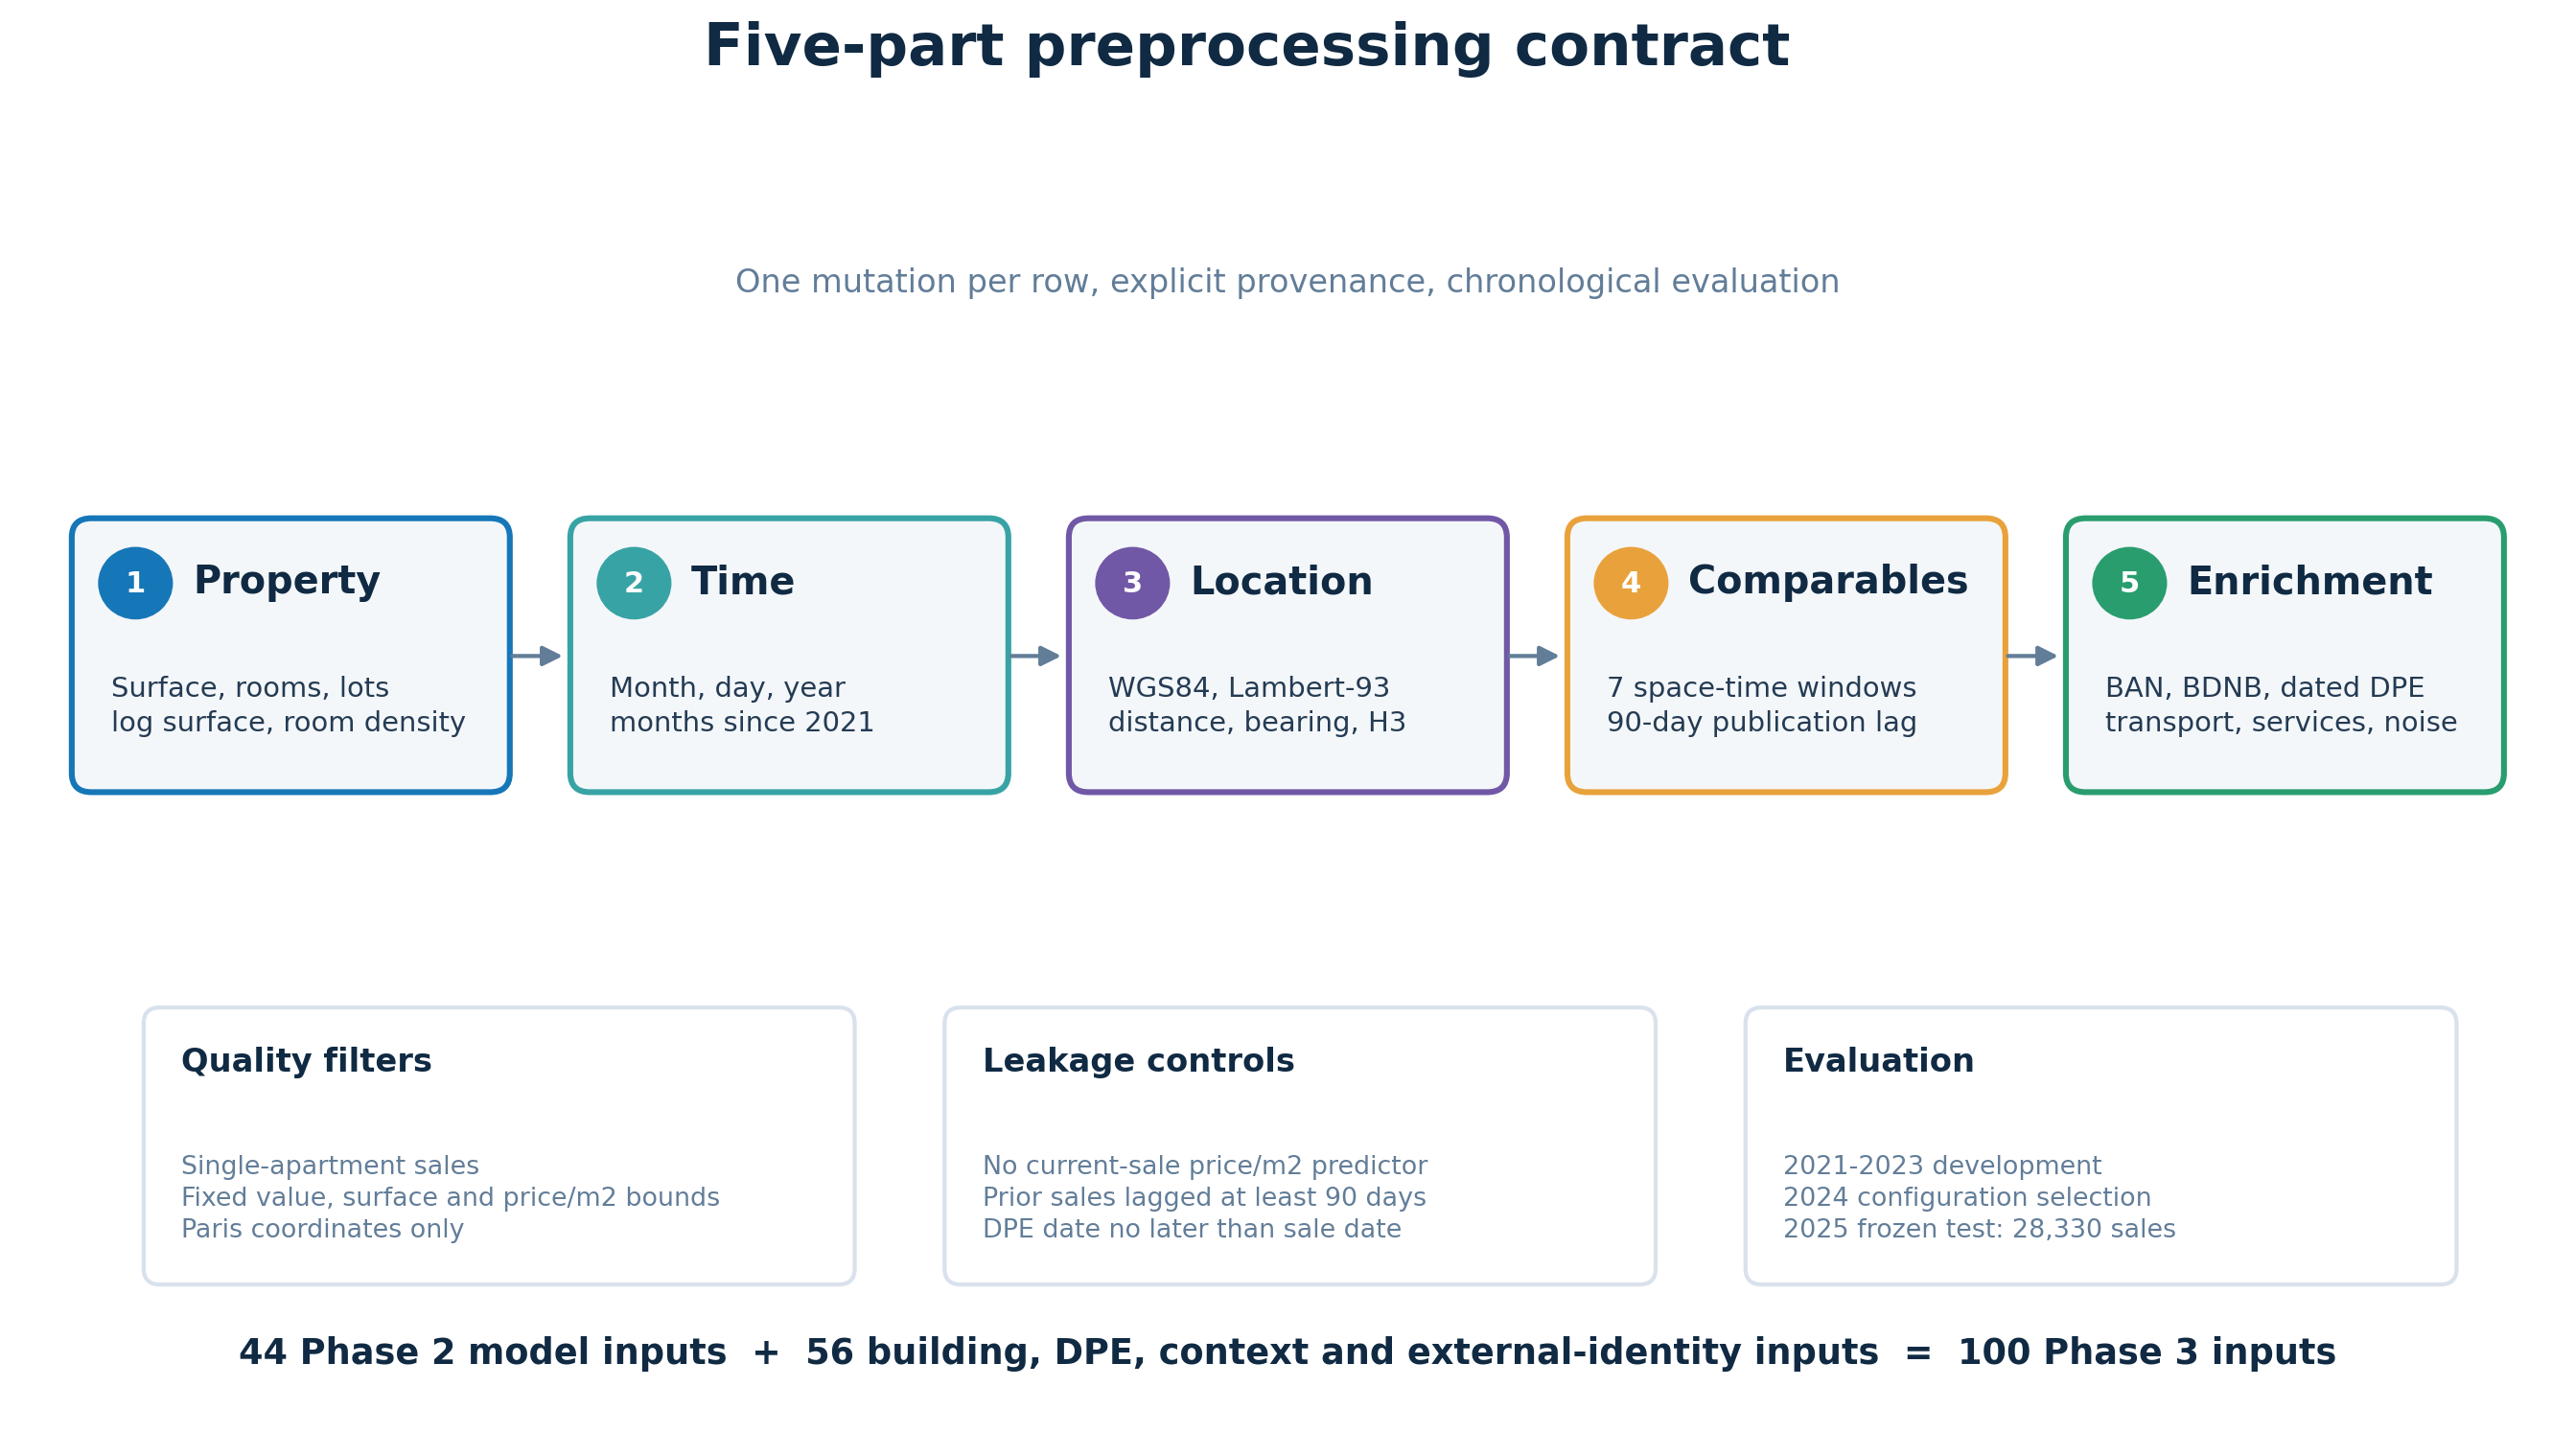
\includegraphics[width=\textwidth]{model_evaluation_feature_contract.png}
\caption{The implemented five-part preprocessing contract and its principal
quality, leakage and evaluation safeguards.}
\label{fig:contract}
\end{figure}

\subsection*{Decision summary}

\begin{itemize}[leftmargin=1.5em]
  \item \textbf{Proceed with the Phase 3 model as the research benchmark.}
  It dominates the frozen Phase 2 reference on MAE, MdAPE, within-20\% accuracy
  and $R^2$.
  \item \textbf{Retain the Phase 2 correction as an operational fallback.}
  It is simpler, transparent and uses only DVF plus lagged market evidence.
  \item \textbf{Do not describe all enrichment as point-in-time.} Dated DPE and
  historical comparables are temporally safe; current BAN/BDNB, transport,
  school, park, service and noise snapshots are retrospective-static context.
  \item \textbf{Monitor price-extreme calibration.} The lowest-value decile is
  overpredicted by EUR 34,507 on average; the highest-value decile is
  underpredicted by EUR 221,745.
  \item \textbf{Seek prospective confirmation.} Aggregate 2025 performance was
  visible during earlier project phases even though Phase 3 fitting and
  selection do not use 2025 rows.
\end{itemize}

\section{Problem definition and analytical cohort}

The target is total transaction value, \texttt{valeur\_fonciere}, for an
ordinary apartment sale in Paris. The unit of analysis is a mutation, not an
individual DVF property line. This distinction prevents a multi-line sale from
duplicating its total price and receiving excessive training weight.

\subsection{Eligibility and quality filters}

The preprocessing retains transactions satisfying all of the following:
\begin{itemize}[leftmargin=1.5em]
  \item mutation nature is \emph{Vente};
  \item exactly one apartment is present and no house or commercial unit is
  included in the same mutation;
  \item transaction date, value, built surface, Paris postcode and coordinates
  are present;
  \item built surface is 9--300 m$^2$;
  \item total value is EUR 50,000--10,000,000;
  \item observed price per m$^2$ is EUR 2,000--30,000;
  \item postcode is 75001--75020 and coordinates lie inside fixed Paris bounds.
\end{itemize}

The current transaction's price per m$^2$ is calculated only for filtering and
as the source value from which \emph{future transactions} may obtain historical
comparable statistics. It is explicitly excluded from the current row's model
inputs.

\subsection{Chronological split}

\begin{table}[H]
\centering
\caption{Fixed chronological cohort and evaluation role.}
\label{tab:splits}
\begin{tabular}{lrrl}
\toprule
Year & Transactions & Cumulative train size & Role \\
\midrule
2021 & 30,397 & 30,397 & Development \\
2022 & 33,080 & 63,477 & Development \\
2023 & 26,798 & 90,275 & Development \\
2024 & 24,404 & 114,679 & Configuration selection \\
2025 & 28,330 & --- & Frozen final test \\
\midrule
Total & 143,009 & --- & Fixed Gold identity \\
\bottomrule
\end{tabular}
\end{table}

No random train/test split is used. Hyperparameters and feature families are
selected on 2024 only. The chosen configuration is then refitted on 2021--2024
and evaluated once on 2025. This rolling-origin design is materially closer to
deployment than a random split in a changing property market.

\section{Five-part feature engineering}

\subsection{1. Property representation}

The core property layer contains built surface, principal-room count, address
number, lot count and available terrain surface. Two derived quantities improve
scale representation: $\log(1+\text{surface})$ and rooms per 10 m$^2$. Surface
remains both raw and transformed because tree models can exploit different
threshold structures. Missing optional room, lot and terrain values remain
explicitly missing for model-native handling; mandatory surface is never
missing after filtering.

\subsection{2. Transaction time}

Calendar variables are month, day of year, year and months elapsed since
January 2021. These variables expose seasonality and broad price-level drift
without using future target aggregates. They are known at valuation time and
therefore satisfy the point-in-time contract.

\subsection{3. Location and spatial identity}

WGS84 longitude/latitude are transformed to Lambert-93 coordinates
(EPSG:2154), allowing Euclidean distances in metres. The pipeline adds distance
from central Paris and sine/cosine bearing. H3 cells at resolutions 8, 9 and 10
support multiscale spatial identity. Resolutions 8 and 9 enter the benchmark;
resolution 10, street, address and parcel IDs remain in Gold for audit and
history rather than unrestricted memorization.

\subsection{4. Historical comparable sales}

For transaction $i$ at date $t_i$, an eligible comparable $j$ must satisfy
\[
  t_i-t_j \geq 90\text{ days}, \qquad
  t_i-t_j \leq w, \qquad
  d(i,j) \leq r,
\]
where $(r,w)$ spans seven windows: 250 m/365 days; 500 m/180, 365 and 730 days;
and 1,000 m/180, 365 and 730 days. Each window produces a count and median price
per m$^2$. Additional variables measure median absolute deviation, nearest prior
sale distance, median comparable age, effective sample size and 180-versus-365
day price momentum.

Distance and time-decayed comparable price is
\[
  \widehat p_i =
  \frac{\sum_{j\in\mathcal C_i}p_j
  \exp(-d_{ij}/350)\exp(-(a_{ij}-90)/240)}
  {\sum_{j\in\mathcal C_i}
  \exp(-d_{ij}/350)\exp(-(a_{ij}-90)/240)}.
\]
A second estimator restricts candidates to 70--130\% of the target surface and
within one principal room when room information exists. The feature builder
was explicitly tested to ensure the current transaction is never its own
comparable and that empty historical neighborhoods produce valid zero counts,
not failed quality reports.

Weighted-comparable coverage is 77.64\% in the initial 2021 cohort because no
earlier project-year history exists. Coverage reaches 100\% from 2022 onward;
the median 2025 transaction has 243 prior sales within 500 m/365 days and 836
within 1,000 m/365 days.

\begin{figure}[H]
\centering
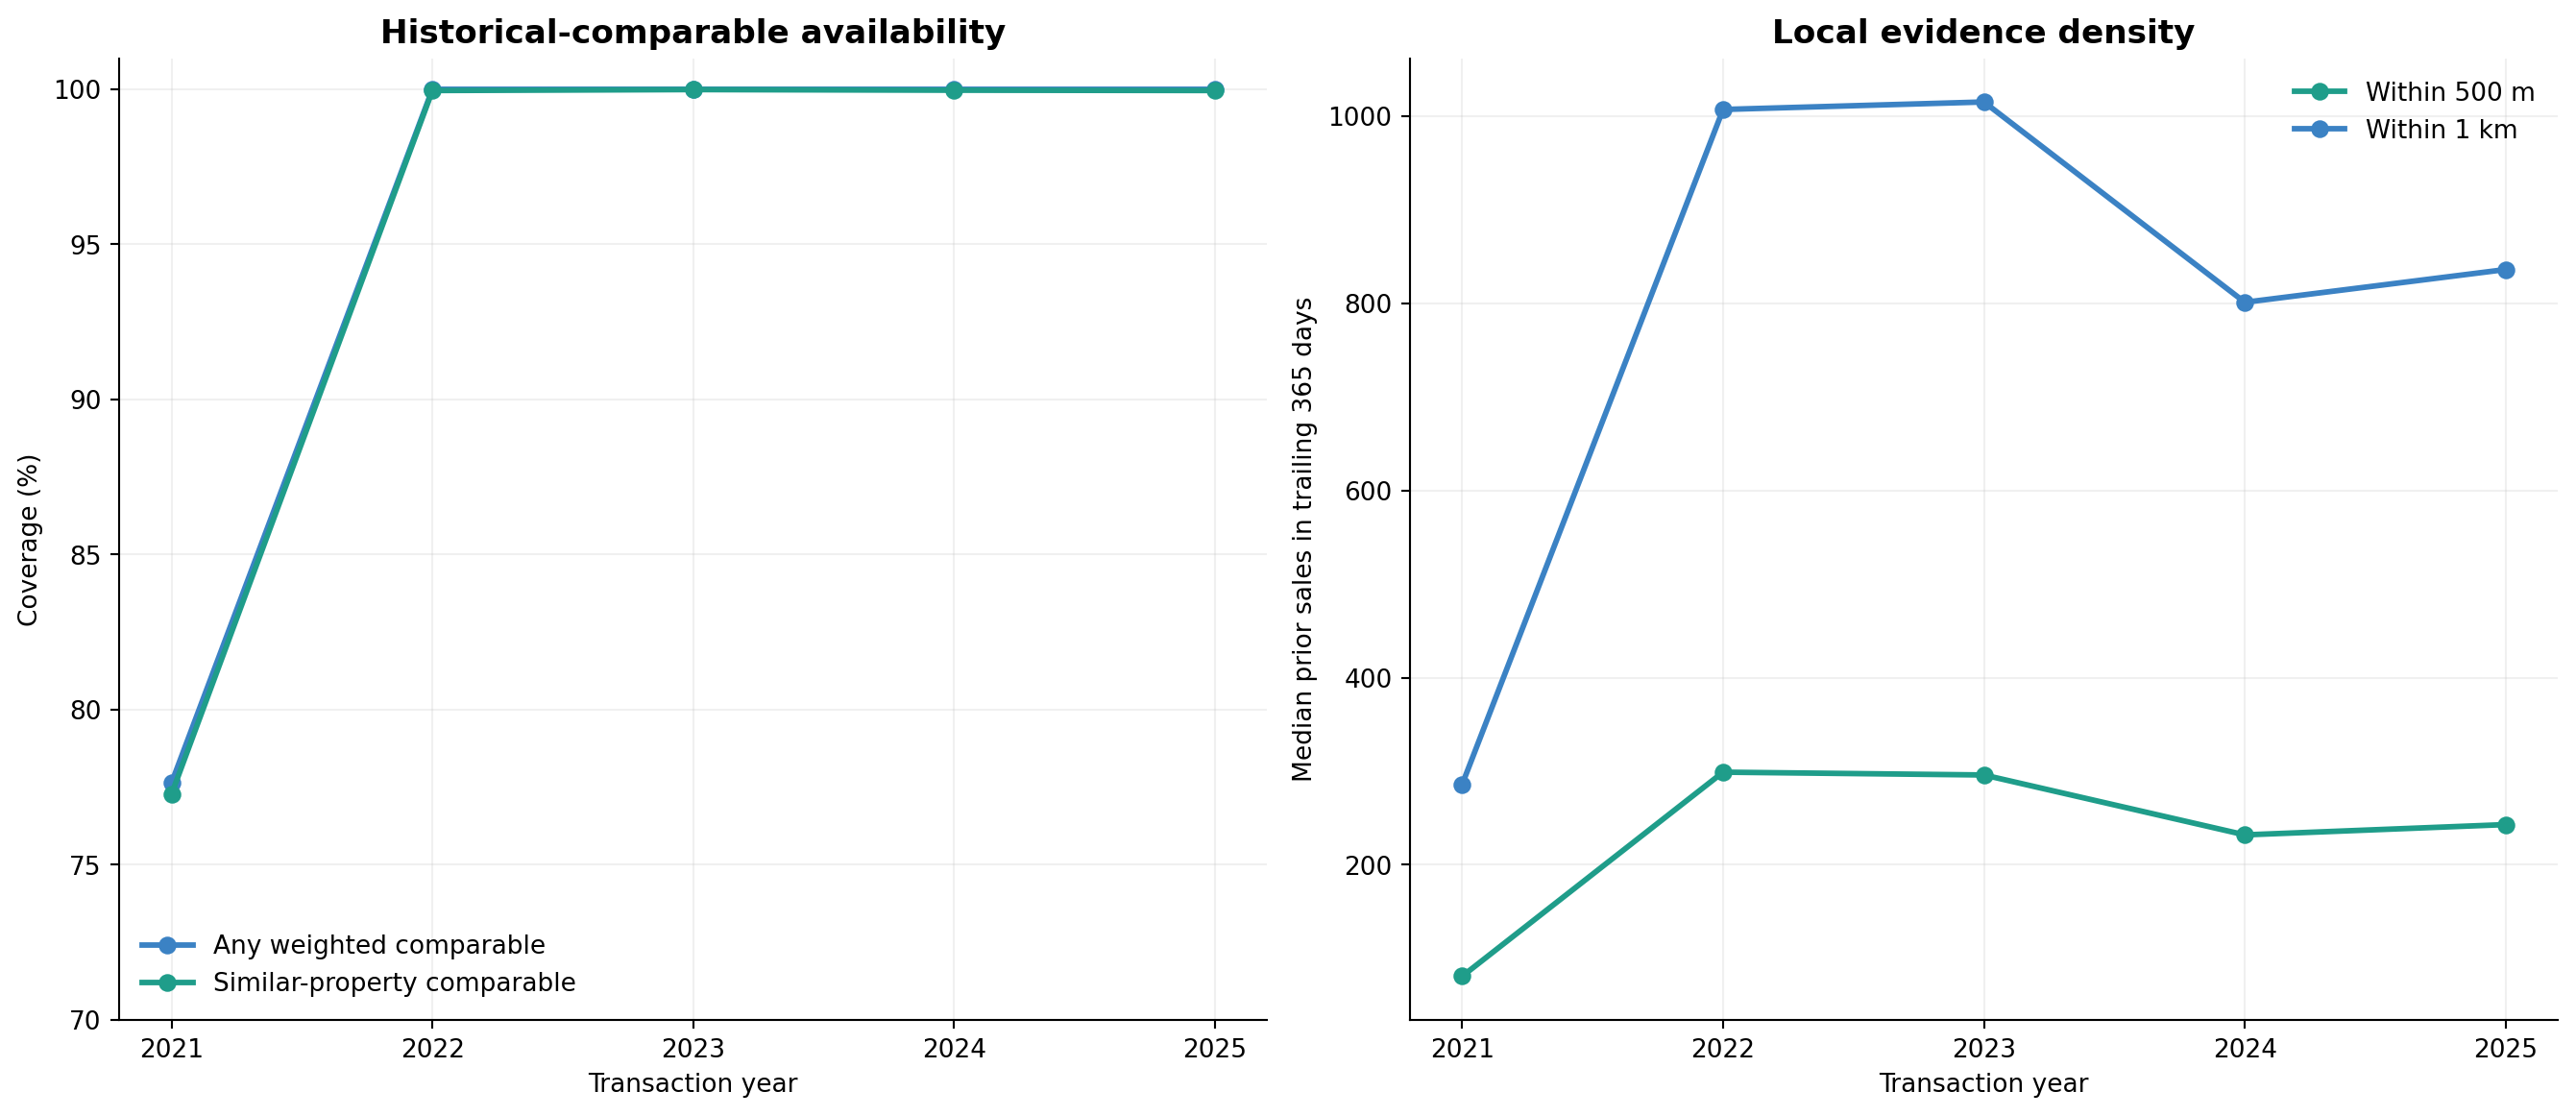
\includegraphics[width=0.94\textwidth]{comparable_coverage.png}
\caption{Historical comparable coverage and density across transaction years.}
\label{fig:compcoverage}
\end{figure}

\subsection{5. Building, energy and neighborhood enrichment}

The external layer links DVF transactions to BAN address identity and BDNB
building identity, then adds physical building attributes, point-in-time DPE,
transport accessibility, schools, parks, services and strategic noise maps.
Exact BAN address resolution covers 99.49\% of transactions; a BDNB building is
resolved for 99.997\%, and 99.46\% receive a high-confidence BDNB match.

Building features include construction year/period, age at sale, level count,
height, footprint, dwelling and lot counts, wall/roof materials, usage and
coarse state. DPE includes energy/GHG classes, consumption, emissions, heating
energy, habitable surfaces, levels and diagnostic-match confidence. Context
features contain distance and density measures for metro, RER, train, tram,
schools, green spaces and services, plus road/RATP/SNCF noise bands.

\begin{figure}[H]
\centering
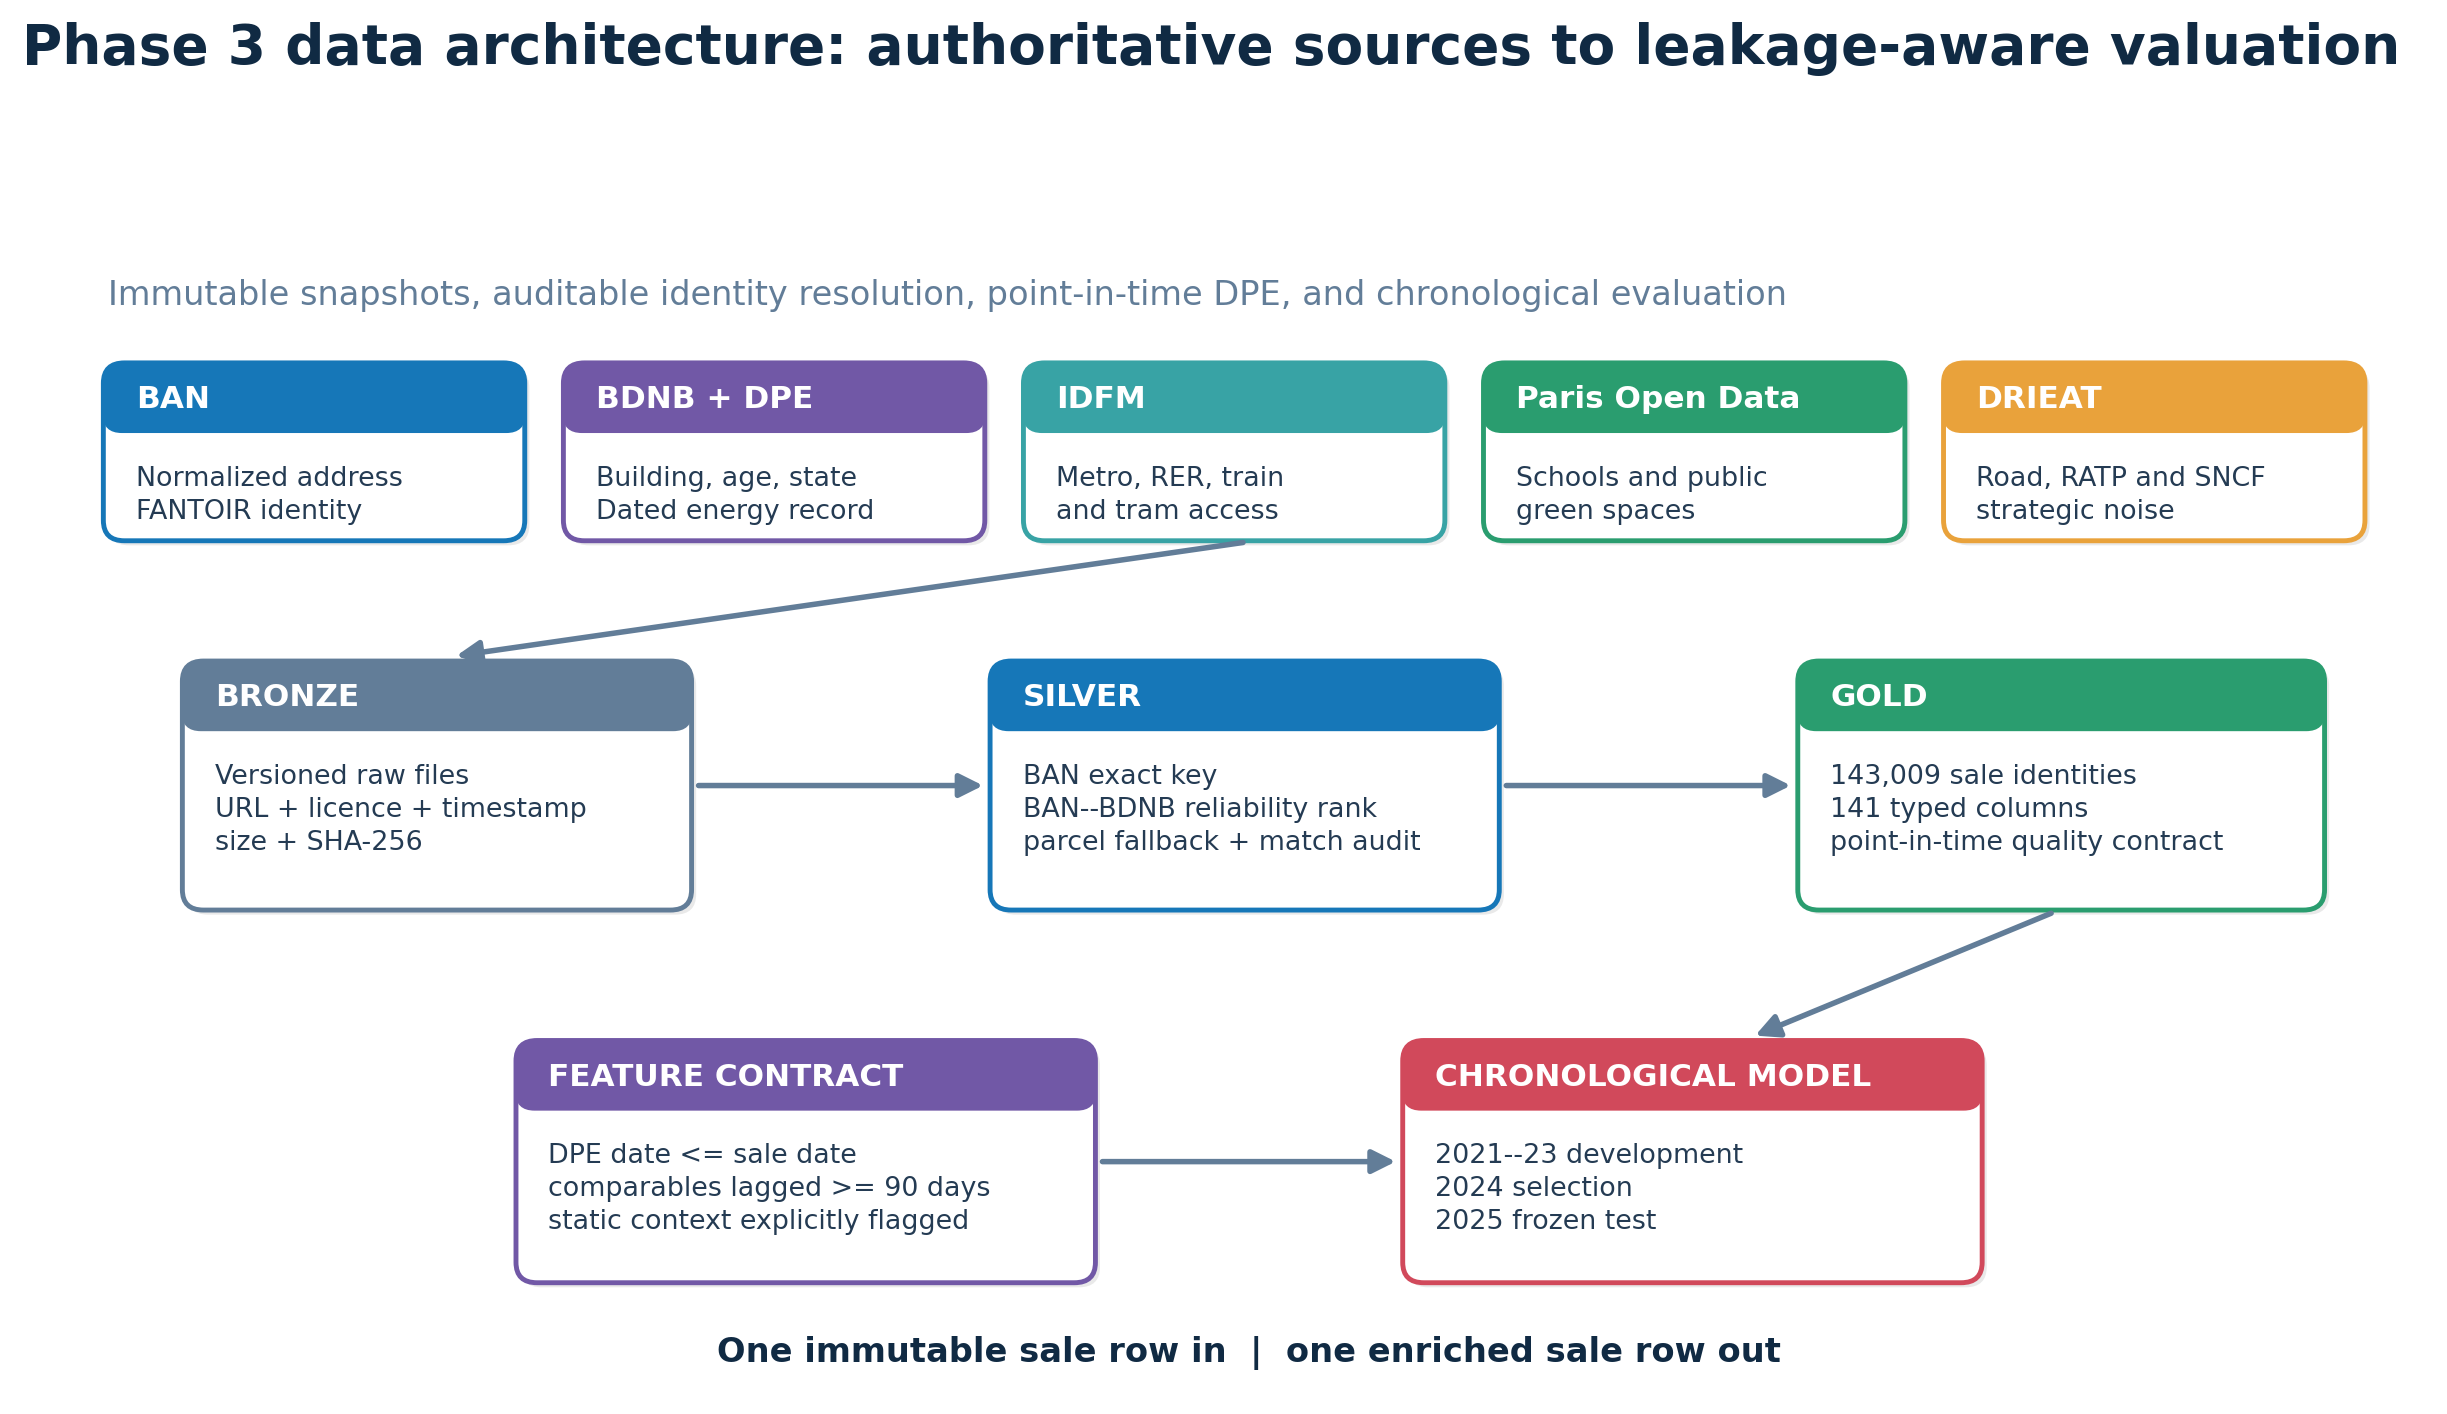
\includegraphics[width=\textwidth]{phase3_data_pipeline.png}
\caption{Bronze--Silver--Gold enrichment architecture. Entity-resolution audit
fields make one-to-many source relationships explicit.}
\label{fig:pipeline}
\end{figure}

\section{Temporal integrity, provenance and validation}

\subsection{Point-in-time versus retrospective-static fields}

Two feature families satisfy strict historical availability:
\begin{enumerate}[leftmargin=1.8em]
  \item historical comparable features, with a minimum 90-day availability
  delay; and
  \item DPE observations whose \texttt{date\_etablissement\_dpe} is no later
  than \texttt{date\_mutation}.
\end{enumerate}
The completed table contains zero future-DPE joins.

BAN/BDNB identity and physical attributes, current transport/school/park/service
locations and the 2022 strategic noise map are retrospective-static context.
They are appropriate for the stated reconstruction experiment but must not be
presented as if every value were available at each historical sale date.

\subsection{Artifact controls}

Each stage publishes atomically: a temporary file is fully written before it
replaces the previous valid artifact. Quality reports record source and output
SHA-256 checksums, row counts, date range, coordinate reference systems,
feature names, comparable coverage, join coverage and missingness. Phase 3
asserts that enrichment preserves row count, order and mutation identity.

The unified command is:
\begin{verbatim}
python -m paris_avm.features.preprocessing
\end{verbatim}
If enrichment is interrupted after Phase 2, \texttt{--reuse-phase2} verifies
the existing Phase 2 checksum before resuming, avoiding an unnecessary
comparable-feature rebuild.

\section{Modeling and statistical protocol}

\subsection{Phase 2 candidates}

Phase 2 evaluates LightGBM and XGBoost on total value, price per m$^2$ and a
residual target, as well as spatial-only and comparable-only ablations. A
validation-selected ensemble is also evaluated. The winning Phase 2 method is
the transparent correction
\[
  \widehat V_i = 0.75\widehat V_i^{\mathrm{LightGBM}}
  + 0.25\left(\widetilde p_{i,365d,500m}\times S_i\right),
\]
where $S_i$ is apartment surface and the local median falls back to the base
prediction when unavailable. It obtains EUR 96,428 MAE and becomes the frozen
reference for Phase 3.

\subsection{Phase 3 candidates and selection}

LightGBM ablations isolate Phase 2, dated DPE, building and neighborhood
families, then combine all enrichment without raw external identity. Both MAE
and Huber objectives are evaluated. CatBoost additionally evaluates the full
100-input contract, including three externally resolved BAN/BDNB identity
fields. Selection uses 2024 validation MAE only.

The selected CatBoost configuration has depth 7, $L_2$ leaf regularization 5
and MAE loss. It is refitted on all 114,679 transactions from 2021--2024 before
producing the 2025 predictions.

\subsection{Metrics and uncertainty}

Reported metrics are MAE, RMSE, $R^2$, mean and median absolute percentage error
(MAPE/MdAPE), and fractions within 10\% and 20\%. MAE confidence intervals use
500 nonparametric bootstrap resamples of 2025 transactions. Improvement
intervals are paired: each resample preserves the Phase 2 and Phase 3 errors of
the same transaction.

\section{Primary model results}

\begin{table}[H]
\centering
\caption{Frozen 2025 performance on 28,330 identical transactions.}
\label{tab:primary}
\small
\begin{tabular}{lrrrrrr}
\toprule
Model & MAE & RMSE & $R^2$ & MdAPE & Within 10\% & Within 20\% \\
\midrule
Phase 2 comparable correction & 96,428 & --- & 0.8601 & 12.22\% & --- & 71.69\% \\
LightGBM, Phase 2 inputs & 95,823 & --- & 0.8630 & --- & --- & --- \\
LightGBM, neighborhood & 95,760 & --- & 0.8637 & --- & --- & --- \\
LightGBM, dated DPE & 95,183 & --- & 0.8634 & --- & --- & --- \\
LightGBM, building & 94,528 & --- & 0.8660 & --- & --- & --- \\
LightGBM, full no identity & 94,204 & --- & 0.8654 & --- & --- & --- \\
\textbf{CatBoost, full 100 inputs} & \textbf{93,197} & \textbf{192,809} & \textbf{0.8679} & \textbf{11.70\%} & \textbf{43.86\%} & \textbf{73.40\%} \\
\bottomrule
\end{tabular}
\end{table}

\begin{figure}[H]
\centering
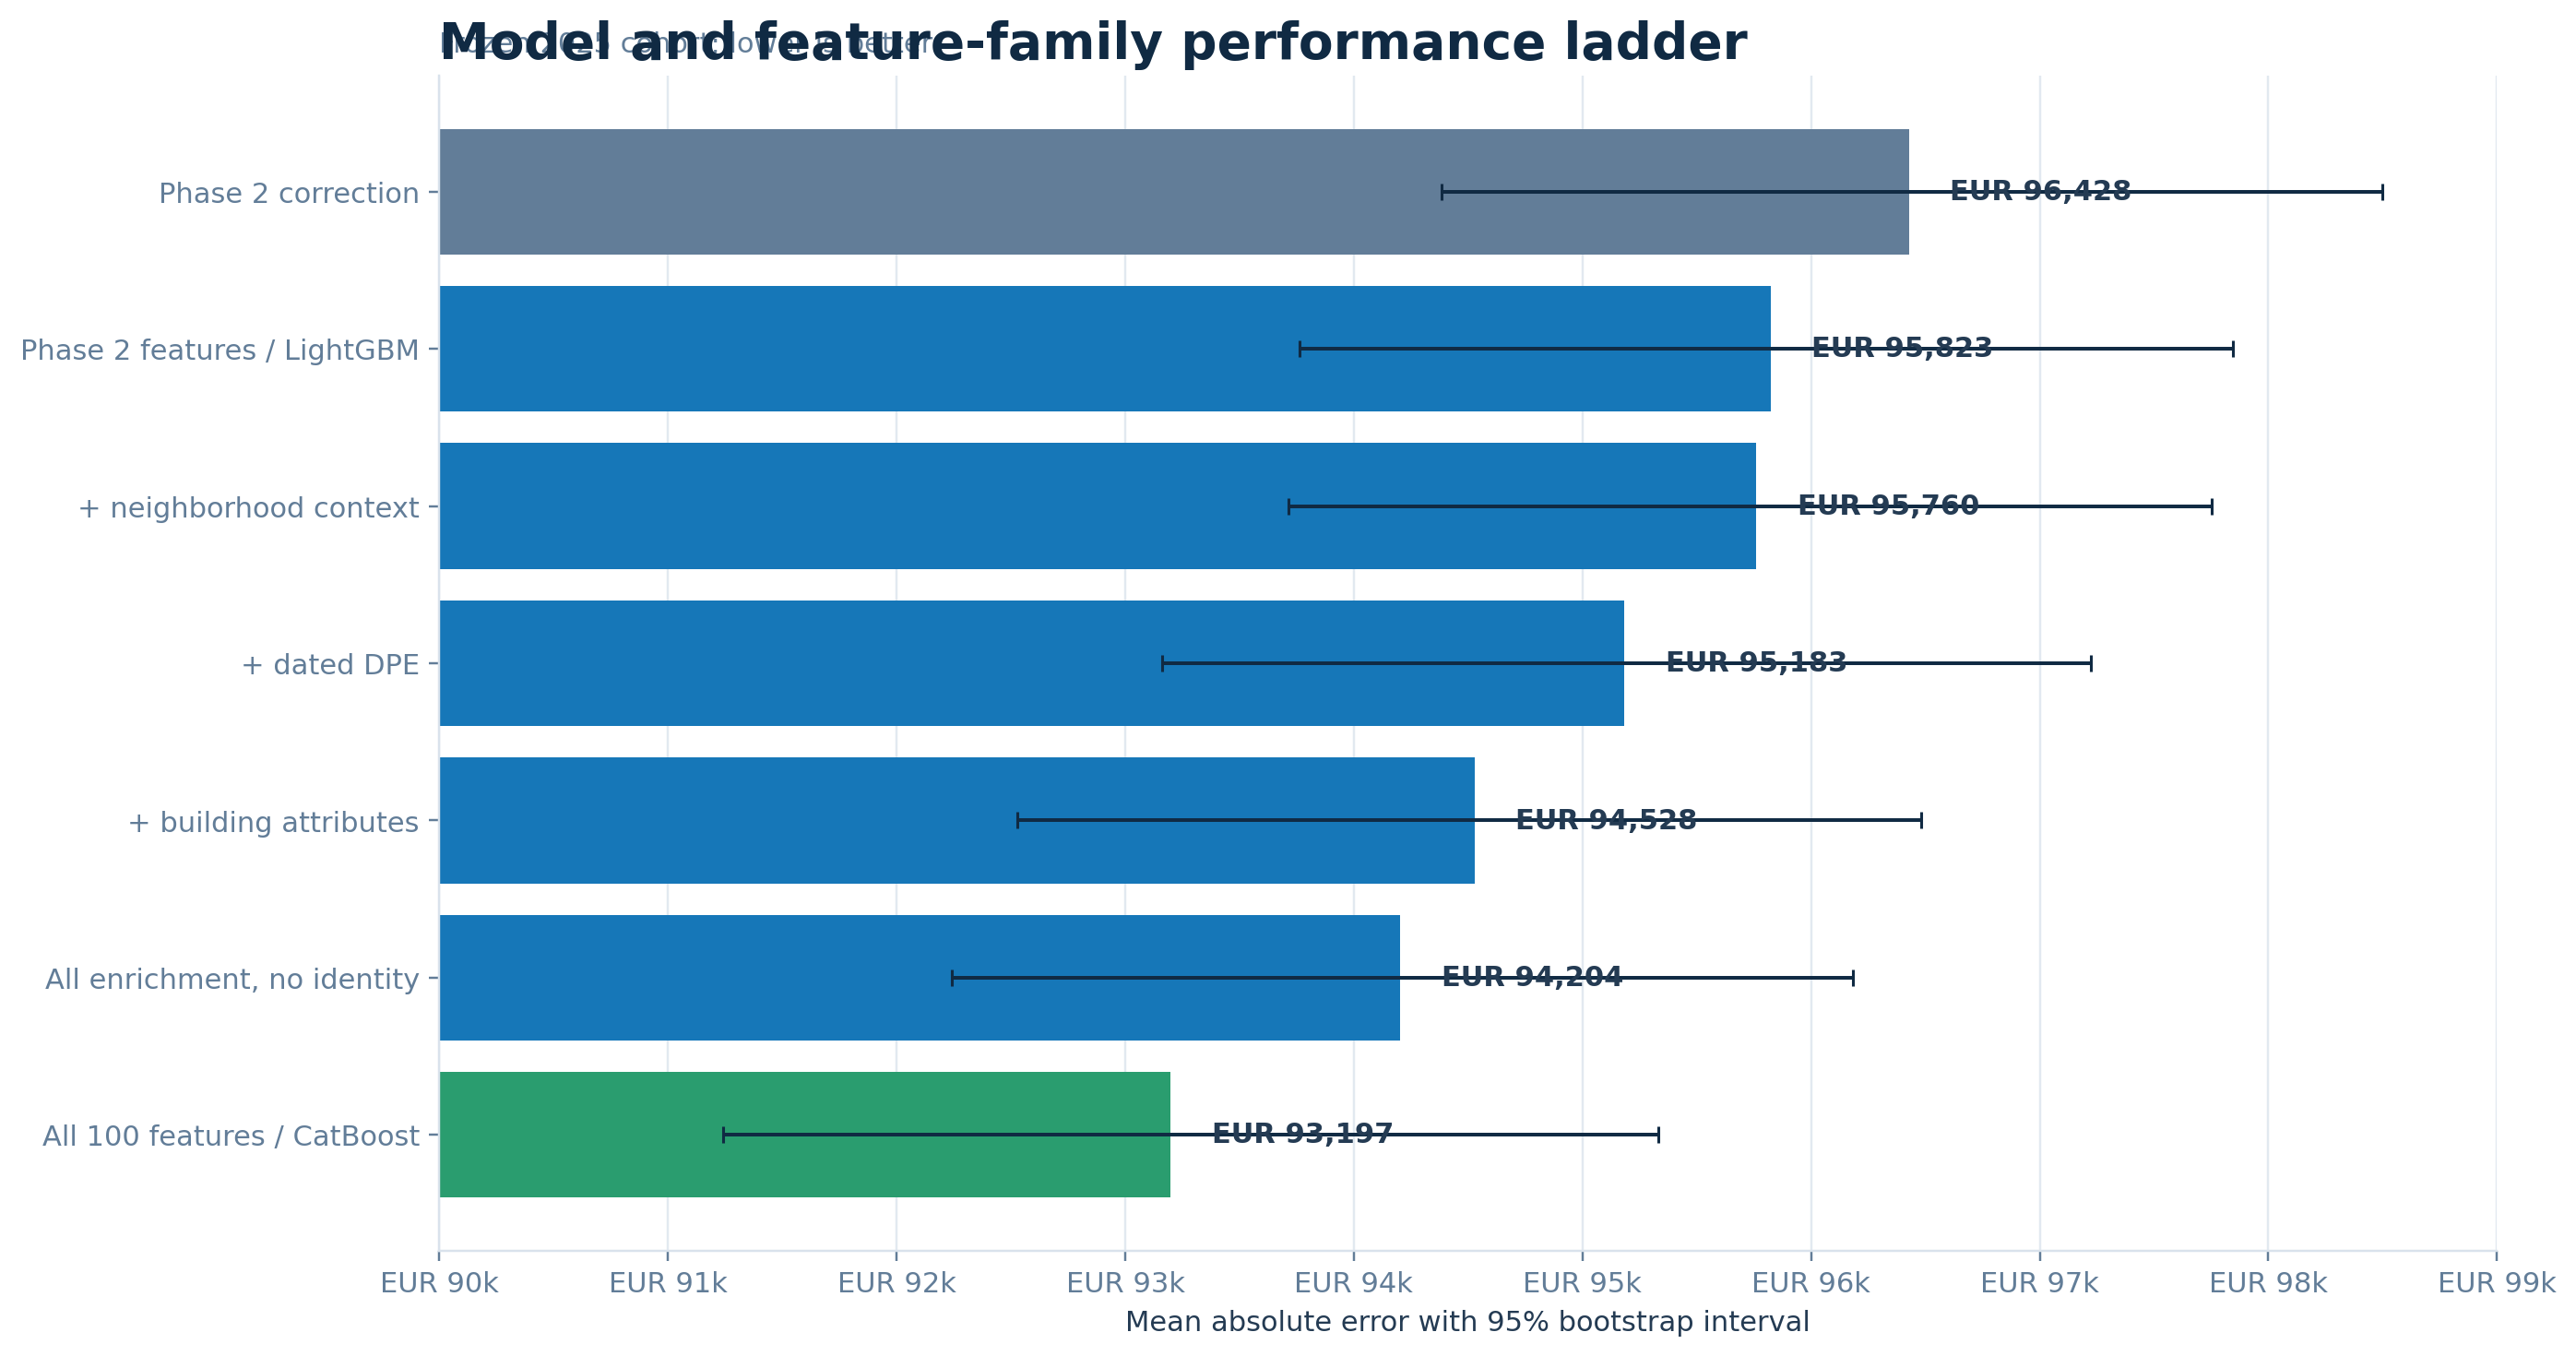
\includegraphics[width=0.94\textwidth]{model_evaluation_performance_ladder.png}
\caption{Selected feature-family and model ladder with 95\% bootstrap intervals.}
\label{fig:ladder}
\end{figure}

The DPE, building and context ablations each outperform the frozen Phase 2
correction, while the combined no-identity model performs better than any
single family. CatBoost with all features improves further. The differences
are predictive associations, not estimates of the market value caused by a
specific building or neighborhood attribute.

\begin{figure}[H]
\centering
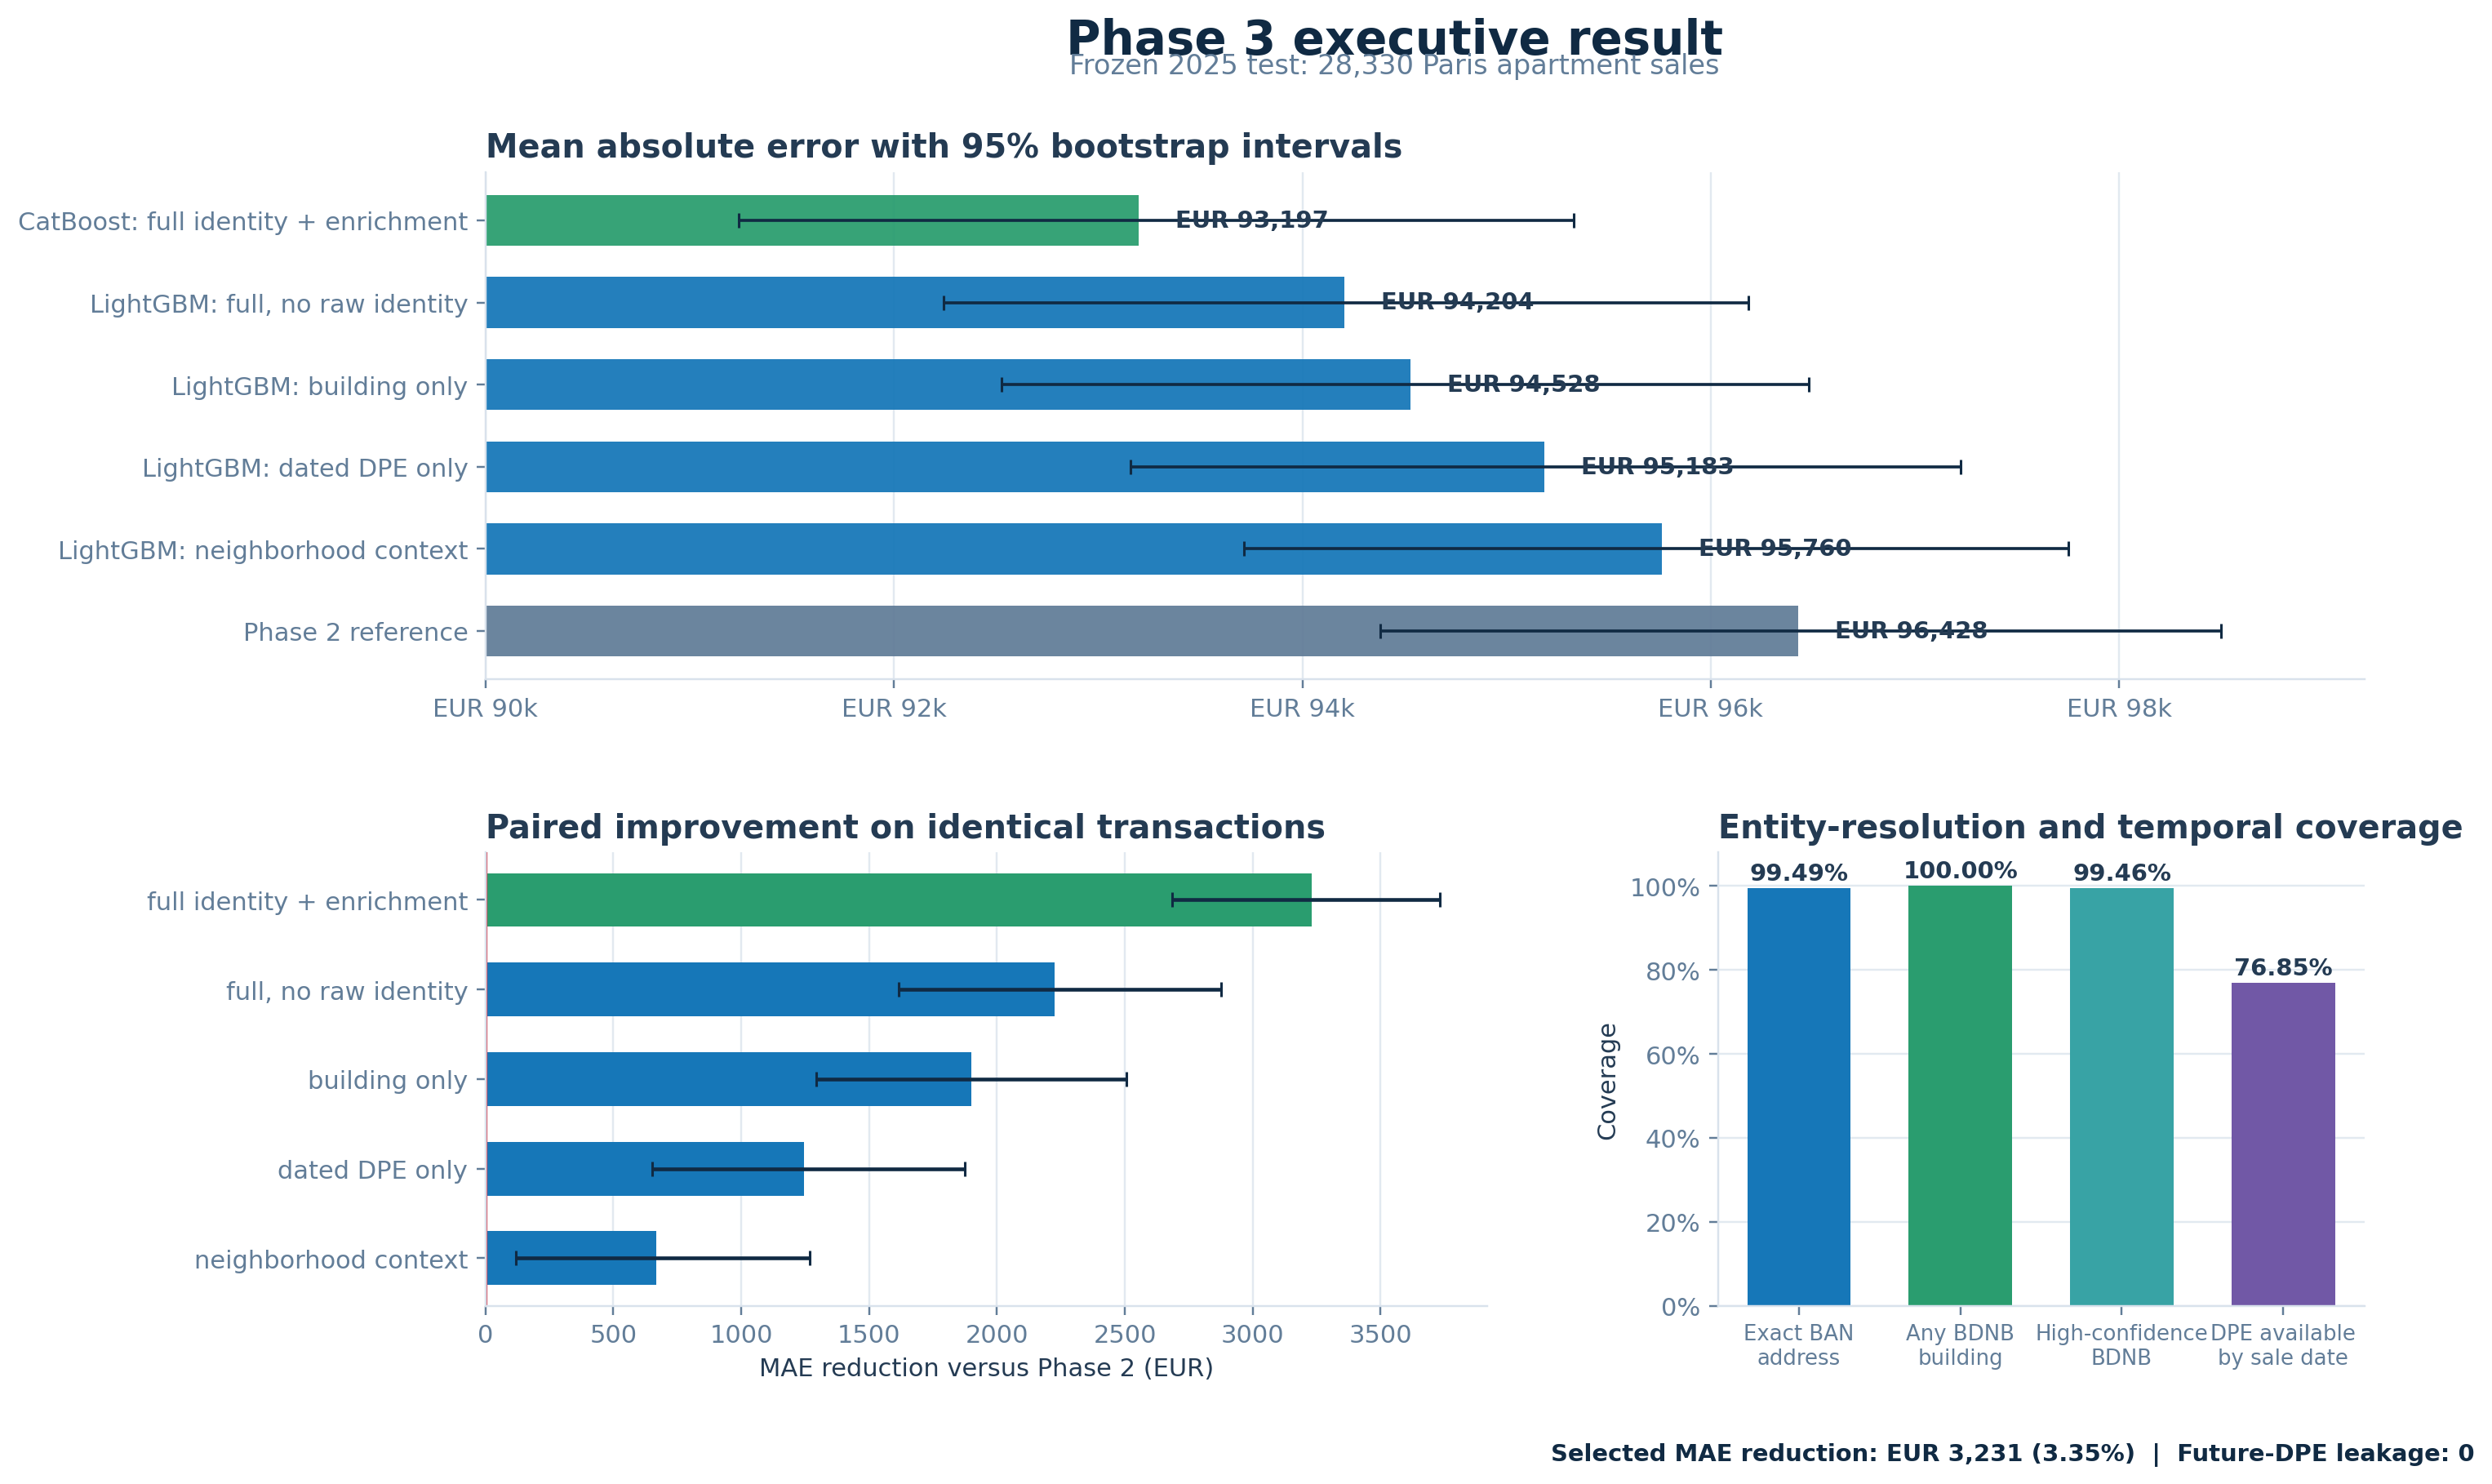
\includegraphics[width=\textwidth]{phase3_results_dashboard.png}
\caption{Executive result, paired improvement intervals and entity-resolution
coverage. The selected MAE reduction is EUR 3,231 (3.35\%).}
\label{fig:dashboard}
\end{figure}

\section{Error analysis and operational robustness}

\subsection{Time and geography}

Phase 3 improves MAE in every month. Monthly reductions range from EUR 1,367
(1.53\%) in May to EUR 5,078 (5.11\%) in October. December is the hardest month
for both systems, with Phase 3 MAE of EUR 101,399; April is the lowest-error
month at EUR 81,428. There is no month in which the enrichment model loses to
the Phase 2 reference.

The gain is also positive in all 20 arrondissements. Absolute reductions are
largest in the 6th (EUR 14,360), 4th (EUR 13,965), 8th (EUR 13,828) and 7th
(EUR 11,718), where transaction values and errors are relatively high. The
smallest reduction is EUR 268 in the 16th. Geography therefore changes the
magnitude of benefit, not its sign on this cohort.

\begin{figure}[H]
\centering
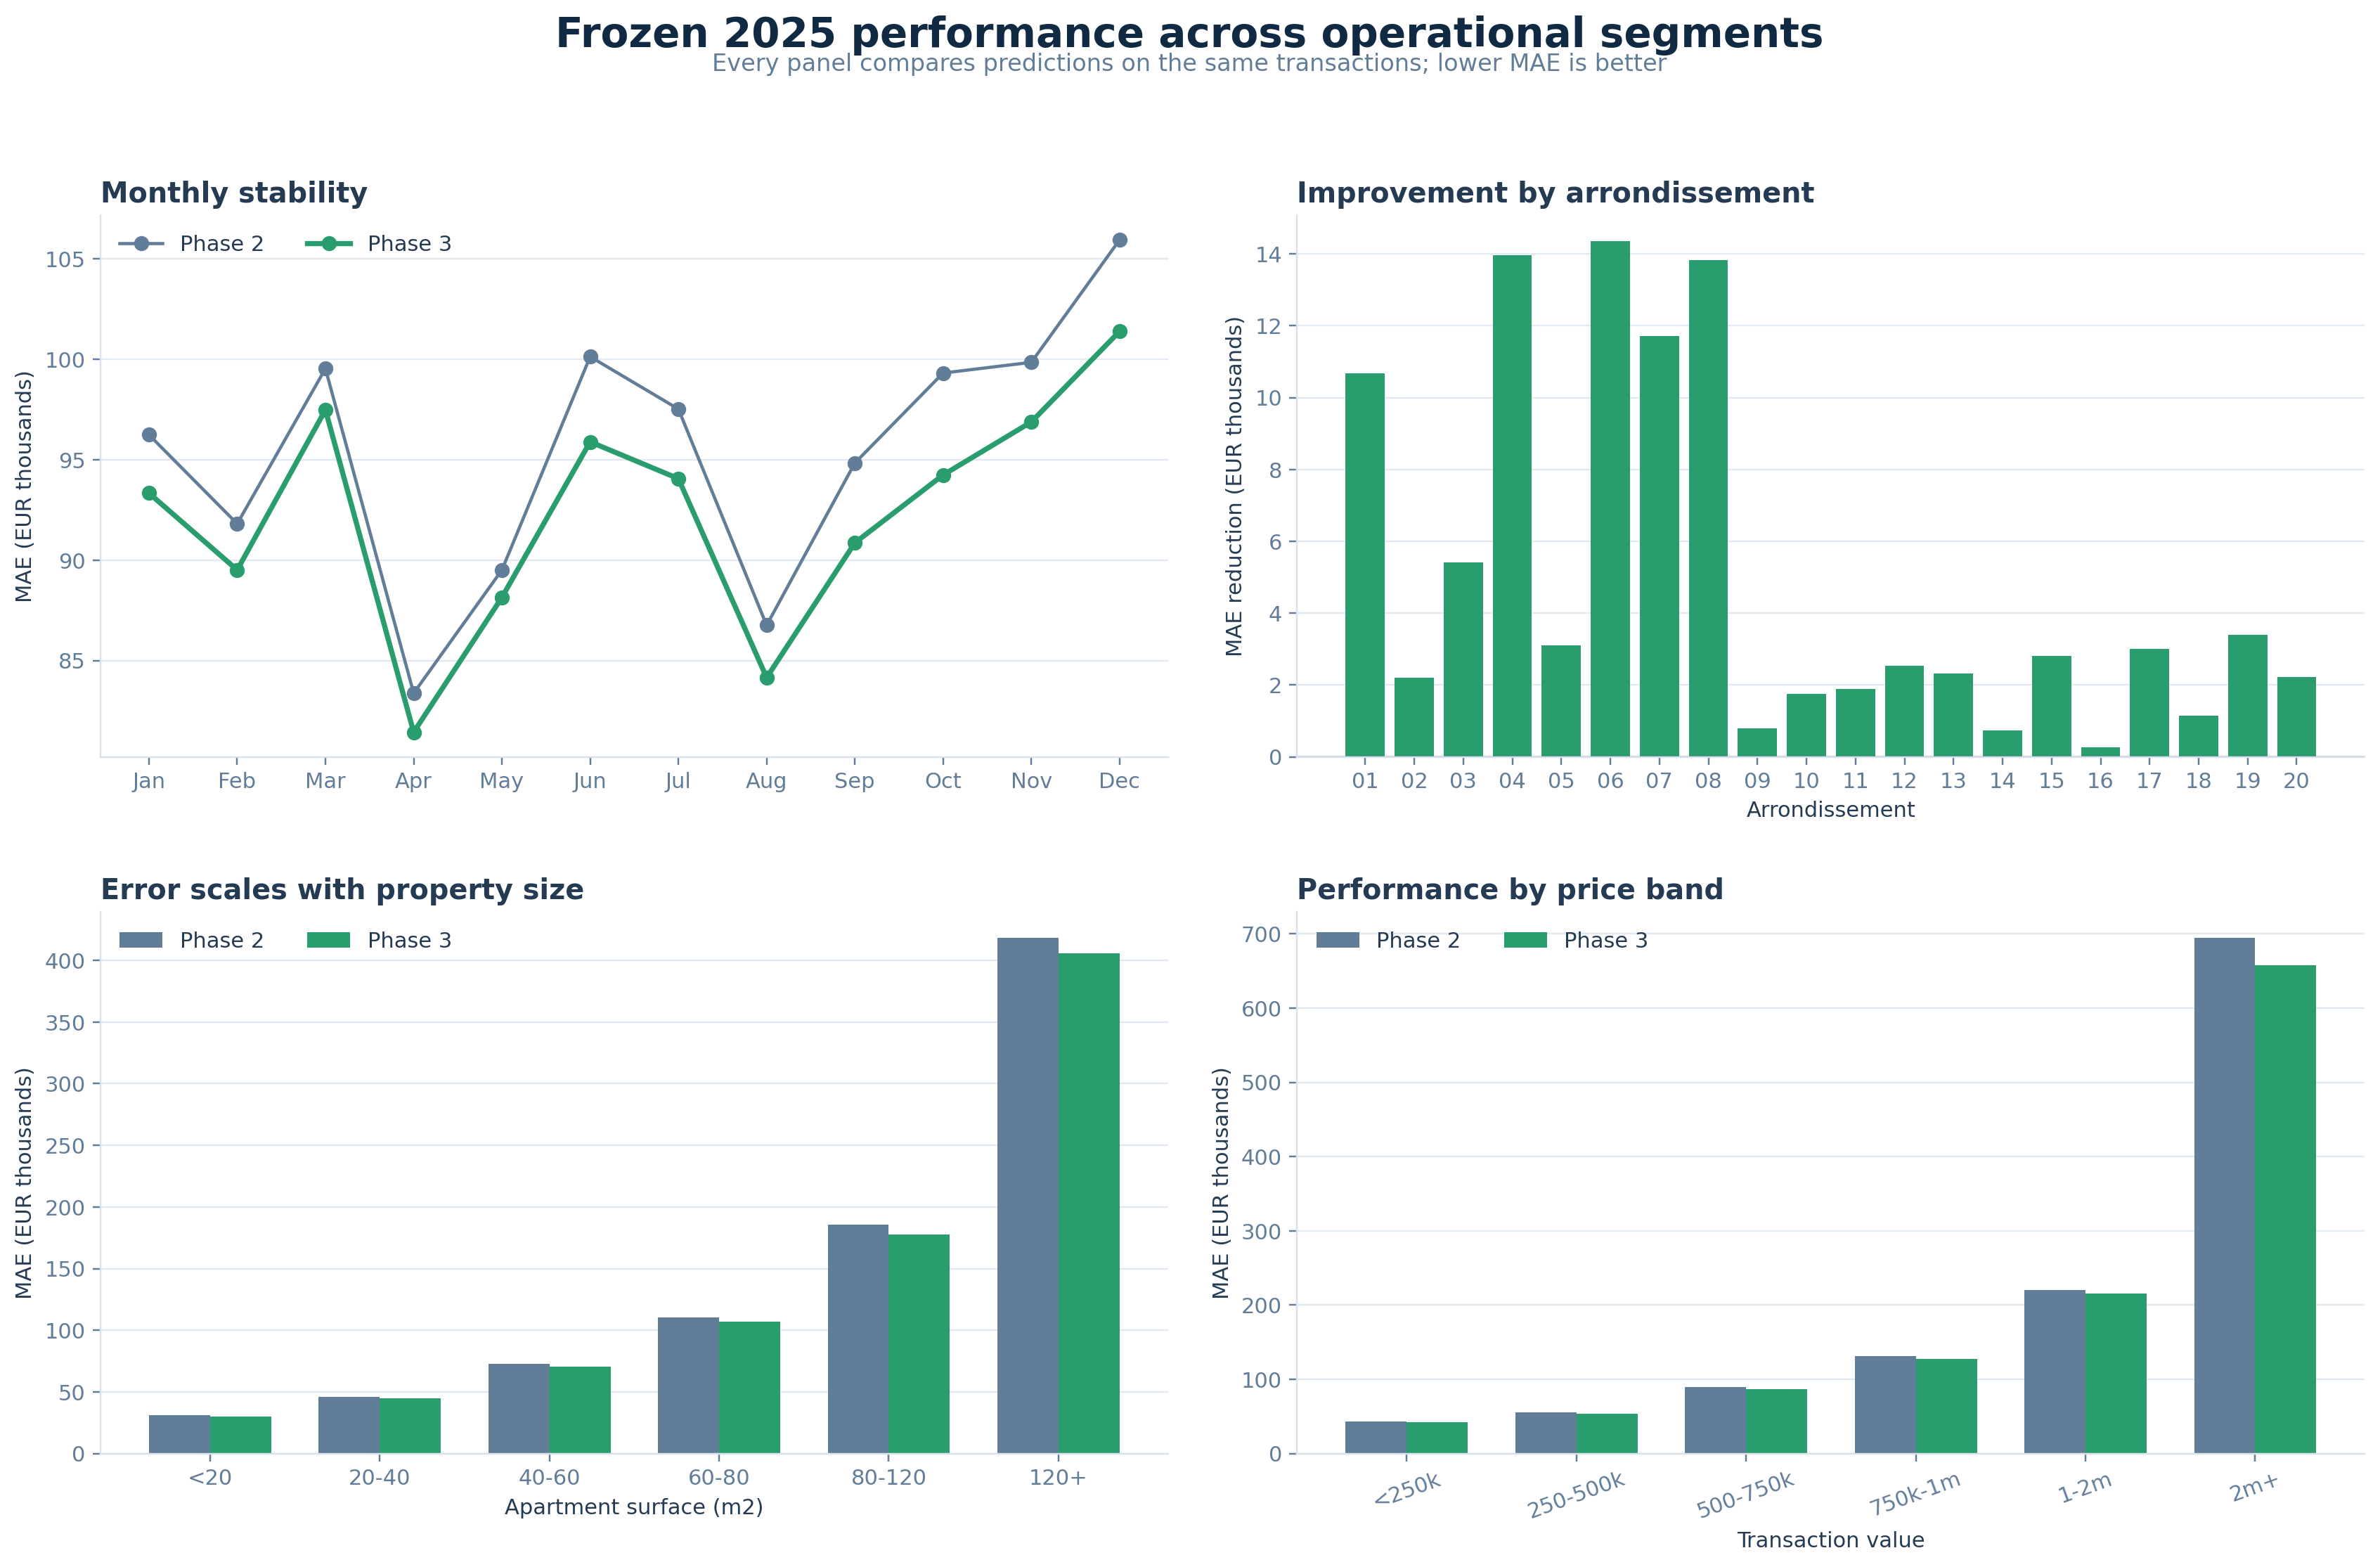
\includegraphics[width=\textwidth]{model_evaluation_segment_dashboard.png}
\caption{Paired Phase 2/Phase 3 diagnostics by month, arrondissement, apartment
surface and transaction-value band.}
\label{fig:segments}
\end{figure}

\subsection{Surface and price bands}

Absolute error scales sharply with property size. Phase 3 MAE is EUR 30,122 for
apartments below 20 m$^2$, EUR 70,564 at 40--60 m$^2$, EUR 177,480 at
80--120 m$^2$, and EUR 405,677 above 120 m$^2$. Enrichment improves every size
band; the largest absolute reduction is EUR 12,670 for the 120+ m$^2$ group.

The same pattern appears by value. Phase 3 MAE is EUR 42,537 below EUR 250,000
and EUR 657,964 above EUR 2 million. The highest-value group improves most in
absolute and relative terms (EUR 36,868; 5.31\%) but retains a 20.43\% MdAPE.
High-value properties remain a distinct operational risk segment.

\subsection{Comparable density and DPE availability}

All 2025 transactions have historical comparable coverage under the broad
1,000 m/730-day definition. Under the tighter 500 m/365-day count, 162 sales
have 1--49 comparables, 9,277 have 50--199, 18,231 have 200--499 and 660 have
500 or more. Phase 3 improves every group. The largest absolute improvement,
EUR 5,026, occurs for the 50--199 group.

Point-in-time DPE is available for 28,140 of 28,330 test sales (99.33\%). The
remaining 190 transactions have much higher Phase 3 MAE (EUR 149,841), partly
because this very small group differs in composition. Phase 3 still improves
both DPE-available and unavailable groups. This comparison is descriptive and
does not isolate a causal DPE contribution.

\begin{figure}[H]
\centering
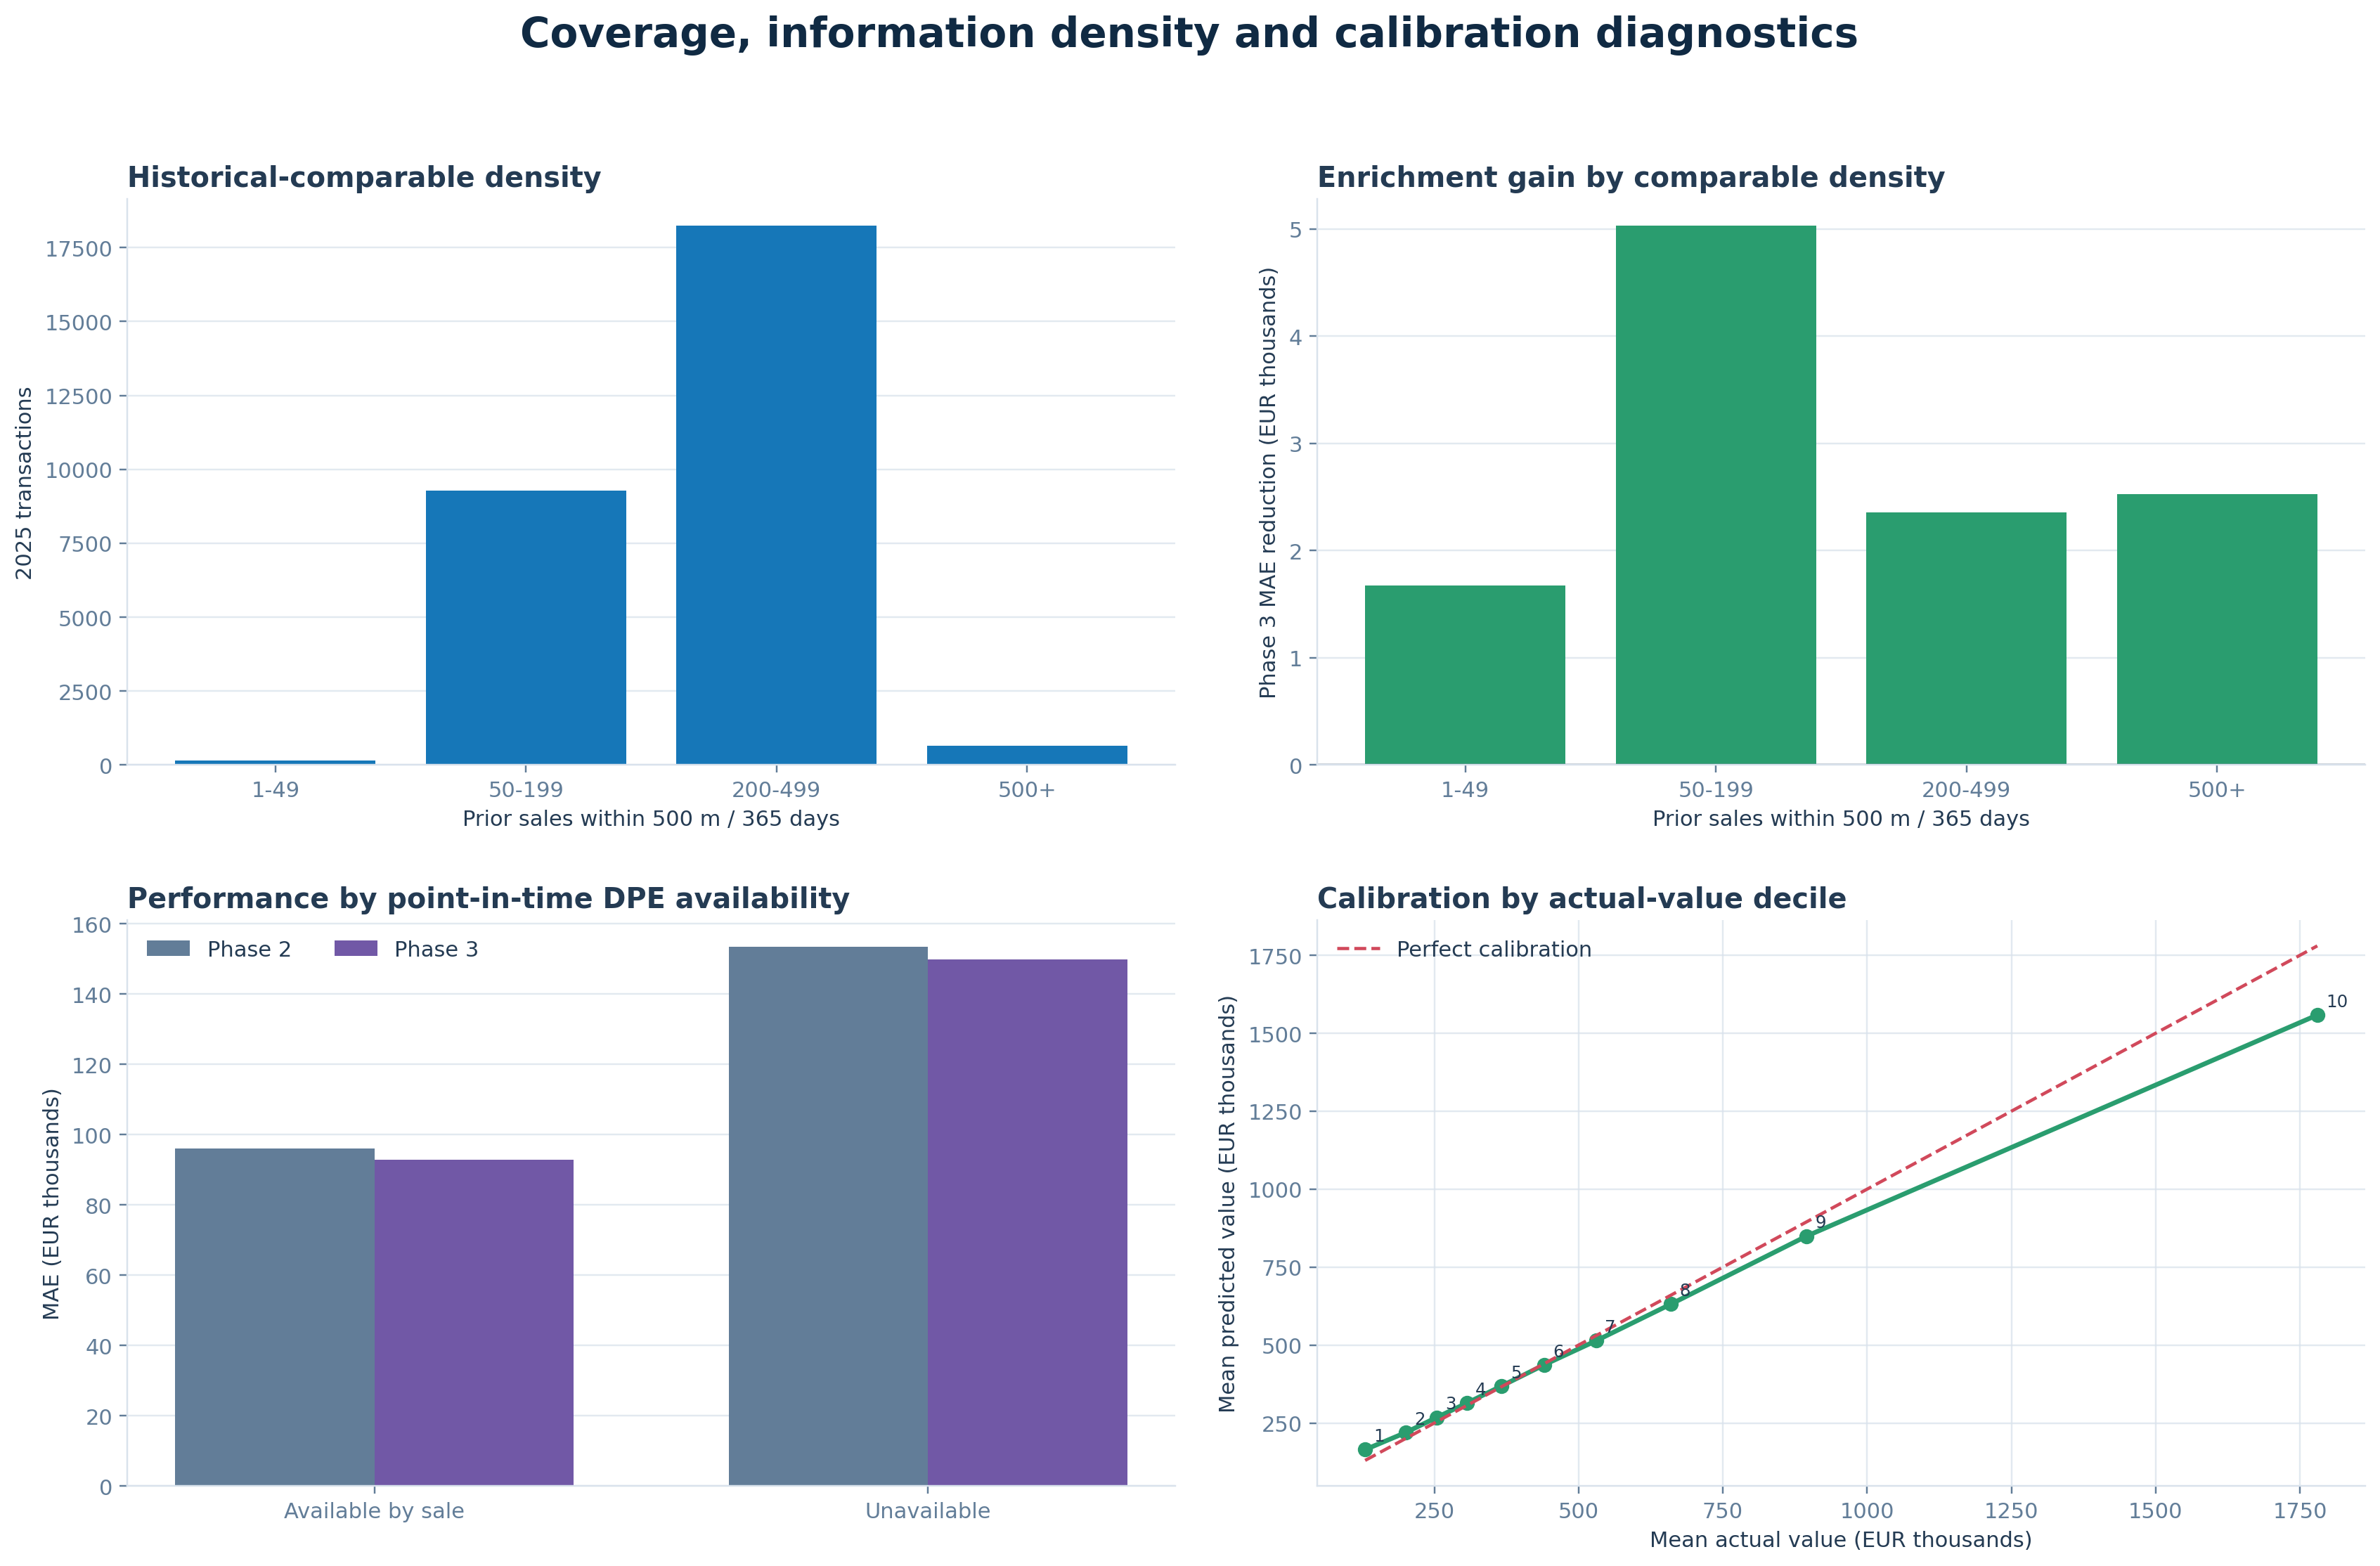
\includegraphics[width=\textwidth]{model_evaluation_coverage_diagnostics.png}
\caption{Comparable density, enrichment gain, DPE availability and
actual-value-decile calibration on the frozen 2025 cohort.}
\label{fig:coveragecalibration}
\end{figure}

\section{Calibration, residuals and spatial behavior}

Average calibration is strongest through the middle of the value distribution.
The lowest decile has mean actual value EUR 130,165 and mean prediction EUR
164,672, an average overprediction of EUR 34,507. Bias changes sign near the
sixth decile. The highest decile has mean actual value EUR 1,780,241 and mean
prediction EUR 1,558,496, an average underprediction of EUR 221,745. This is the
familiar regression-to-the-mean pattern and motivates segment-aware monitoring
or a validation-fitted calibration layer.

\begin{figure}[H]
\centering
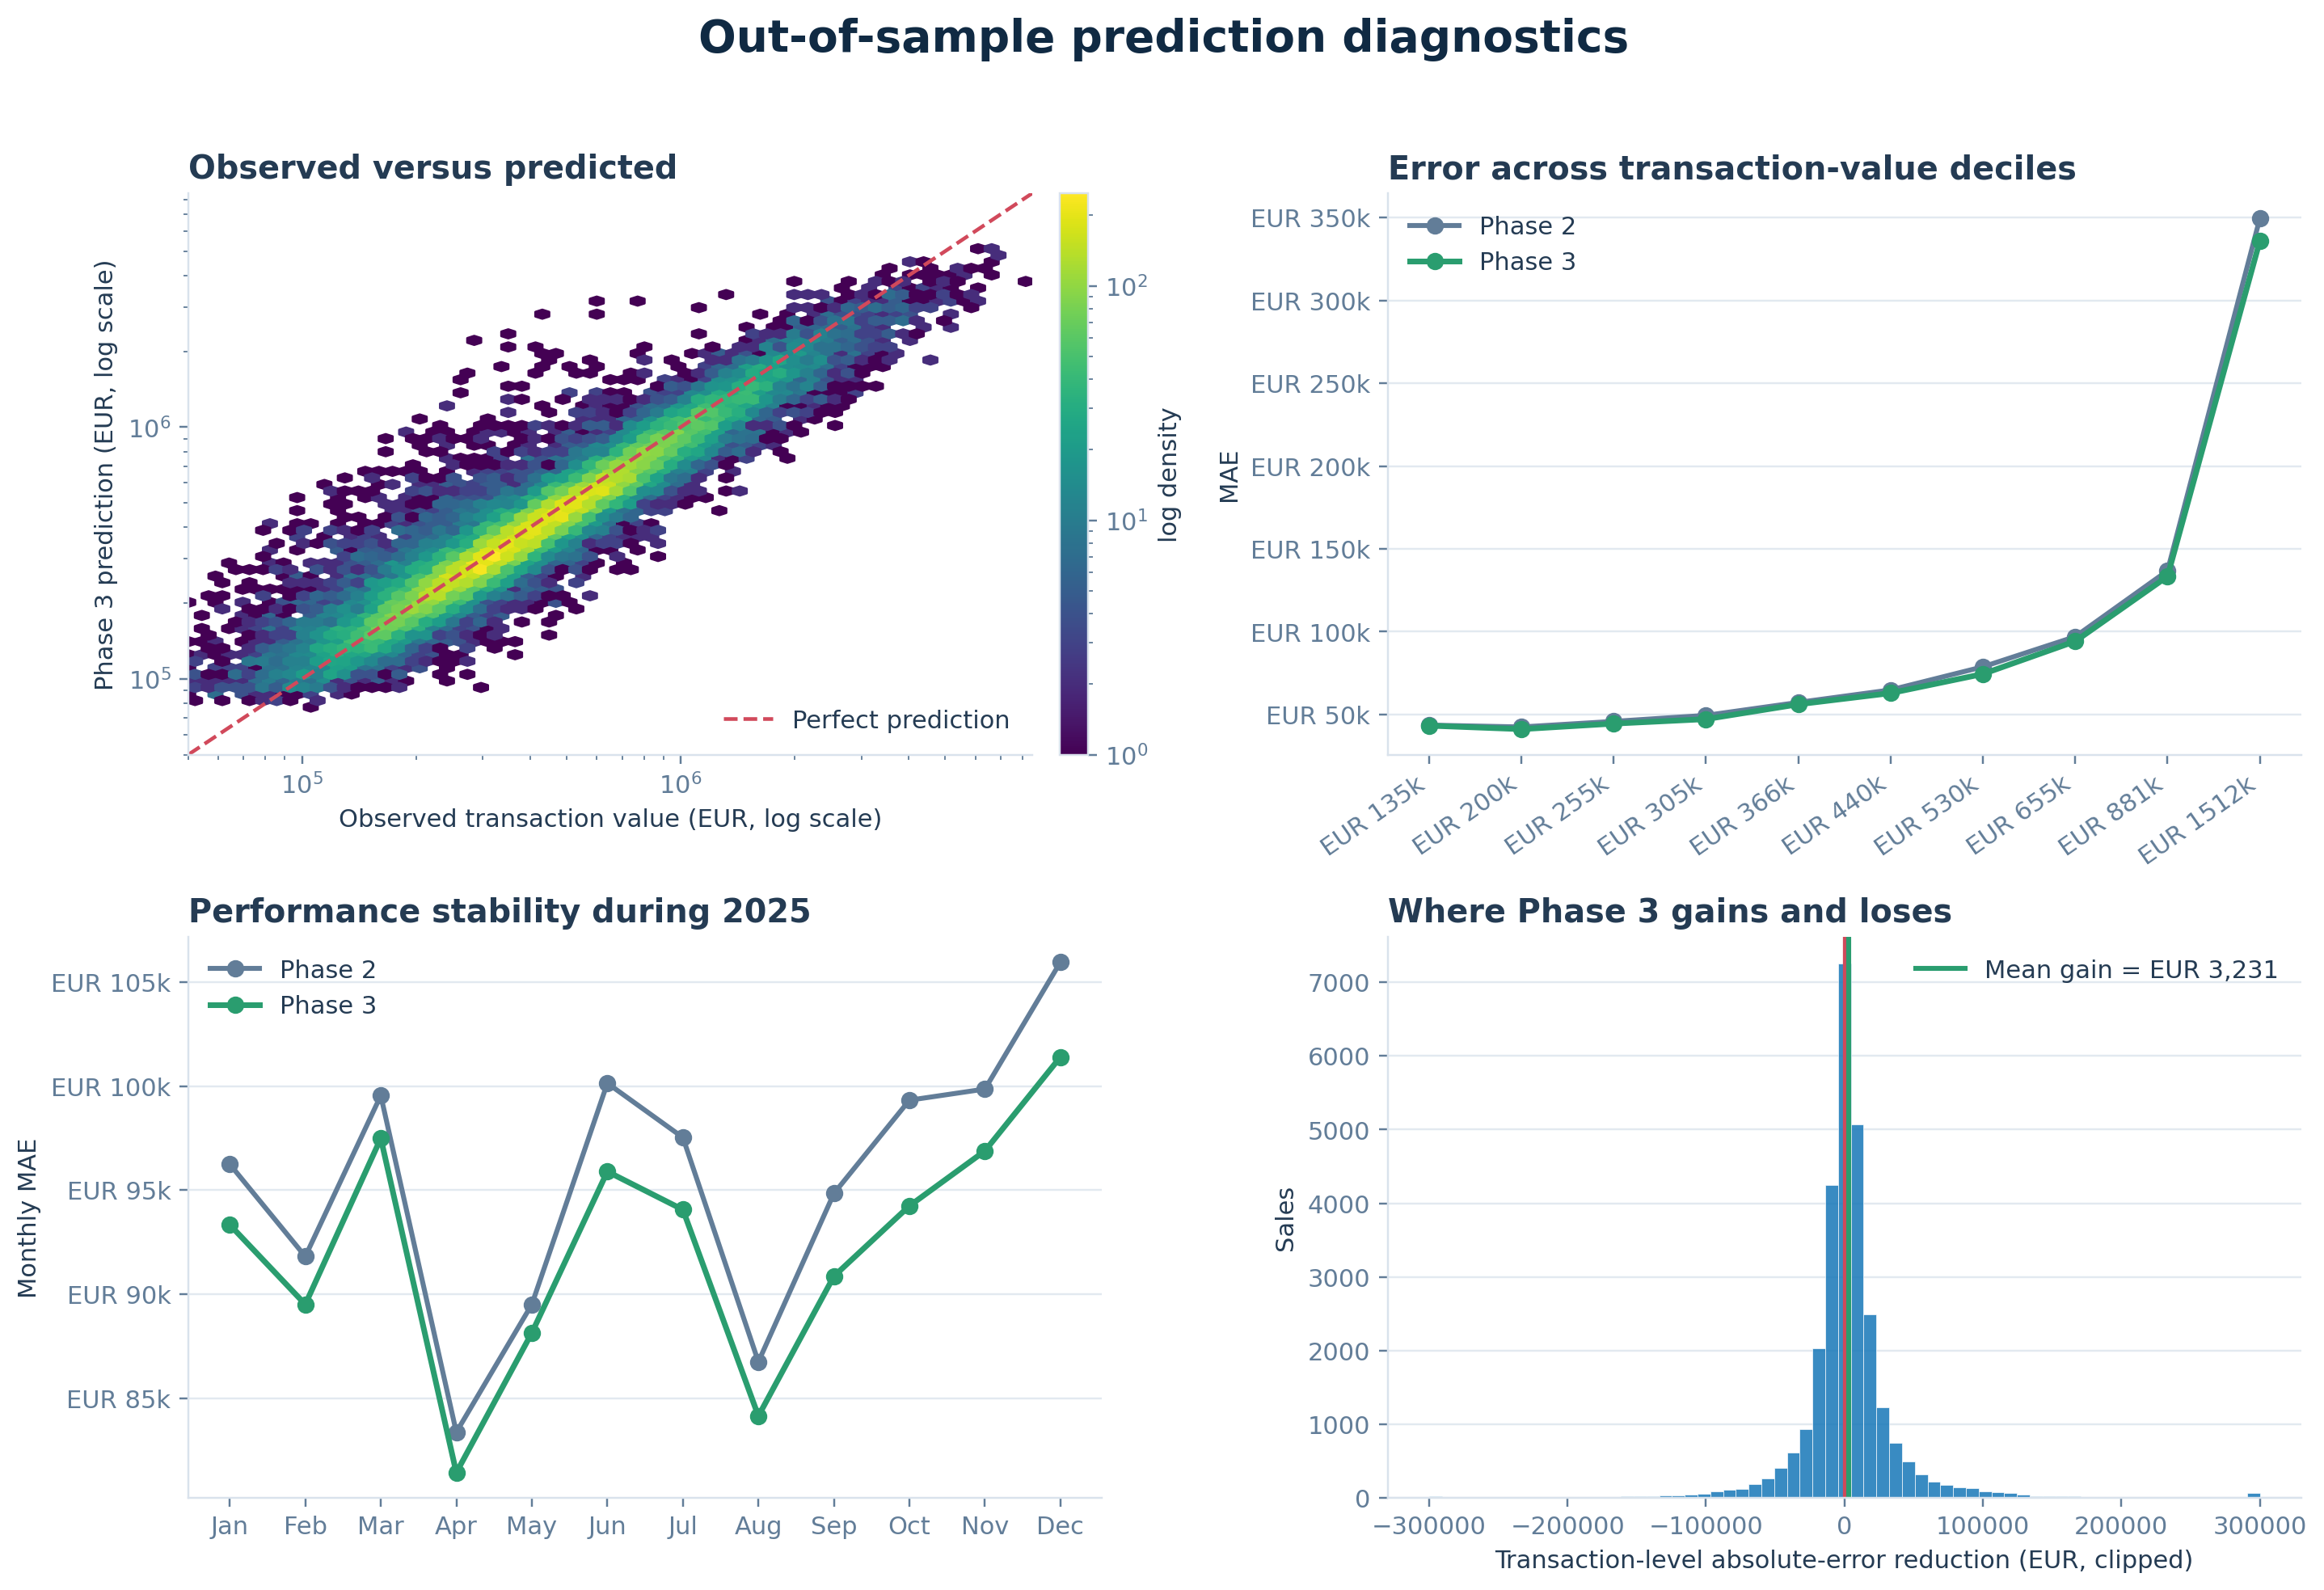
\includegraphics[width=\textwidth]{phase3_prediction_diagnostics.png}
\caption{Out-of-sample prediction, residual, monthly and cumulative-error
diagnostics for the selected model and frozen reference.}
\label{fig:predictiondiagnostics}
\end{figure}

\begin{figure}[H]
\centering
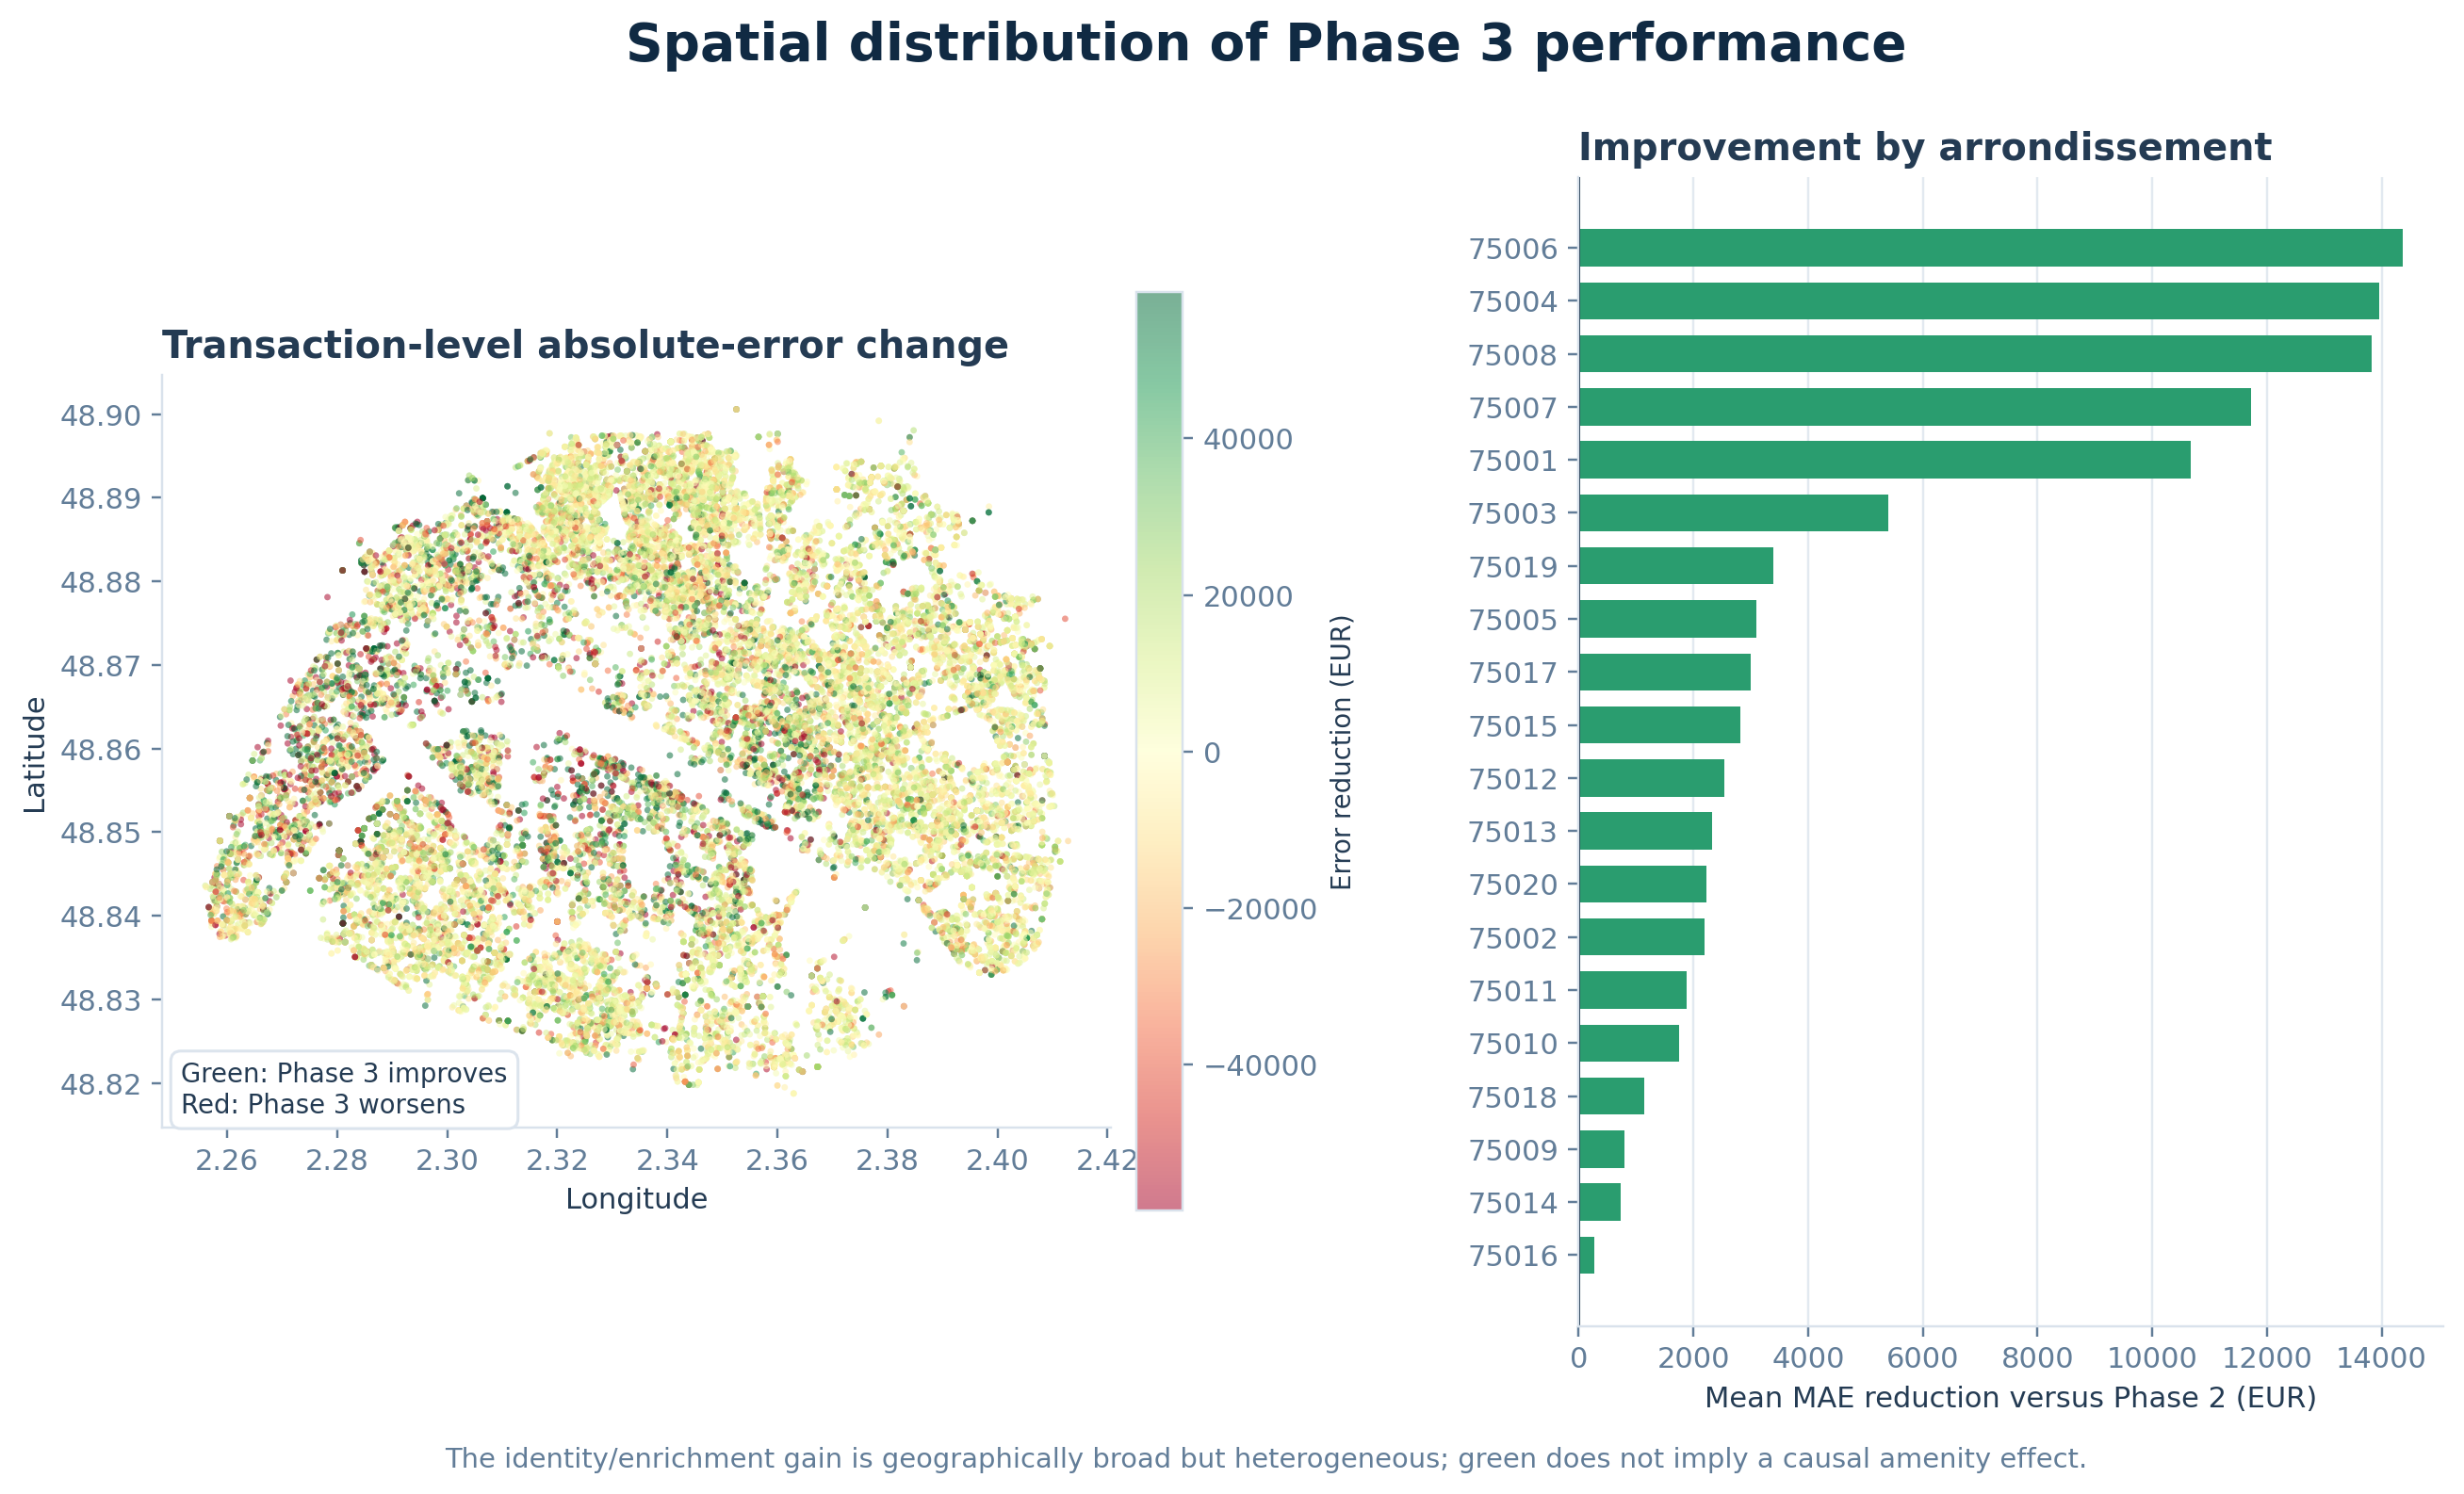
\includegraphics[width=\textwidth]{phase3_spatial_performance.png}
\caption{Spatial distribution of error and paired improvement across Paris.}
\label{fig:spatial}
\end{figure}

\section{Feature importance and interpretation}

CatBoost prediction-value-change importance attributes 79.57\% of total
importance to core DVF/spatial inputs and 12.95\% to historical comparables.
Building/linkage, neighborhood context, DPE/energy and micro-location identity
account for 2.39\%, 2.07\%, 1.86\% and 1.16\%, respectively. The model therefore
remains primarily a surface-and-market-evidence system; enrichment supplies
smaller refinements that collectively improve generalization.

The two dominant individual features are log surface (37.92\%) and raw surface
(35.28\%). The strongest historical signals are 365-day/500-m local median
price per m$^2$, the 365-day/250-m median, similar-comparable price and the
weighted comparable estimate. DPE habitable surface is the highest-ranked DPE
field. Importance is not causal and correlated features divide credit in a
model-dependent manner.

\begin{figure}[H]
\centering
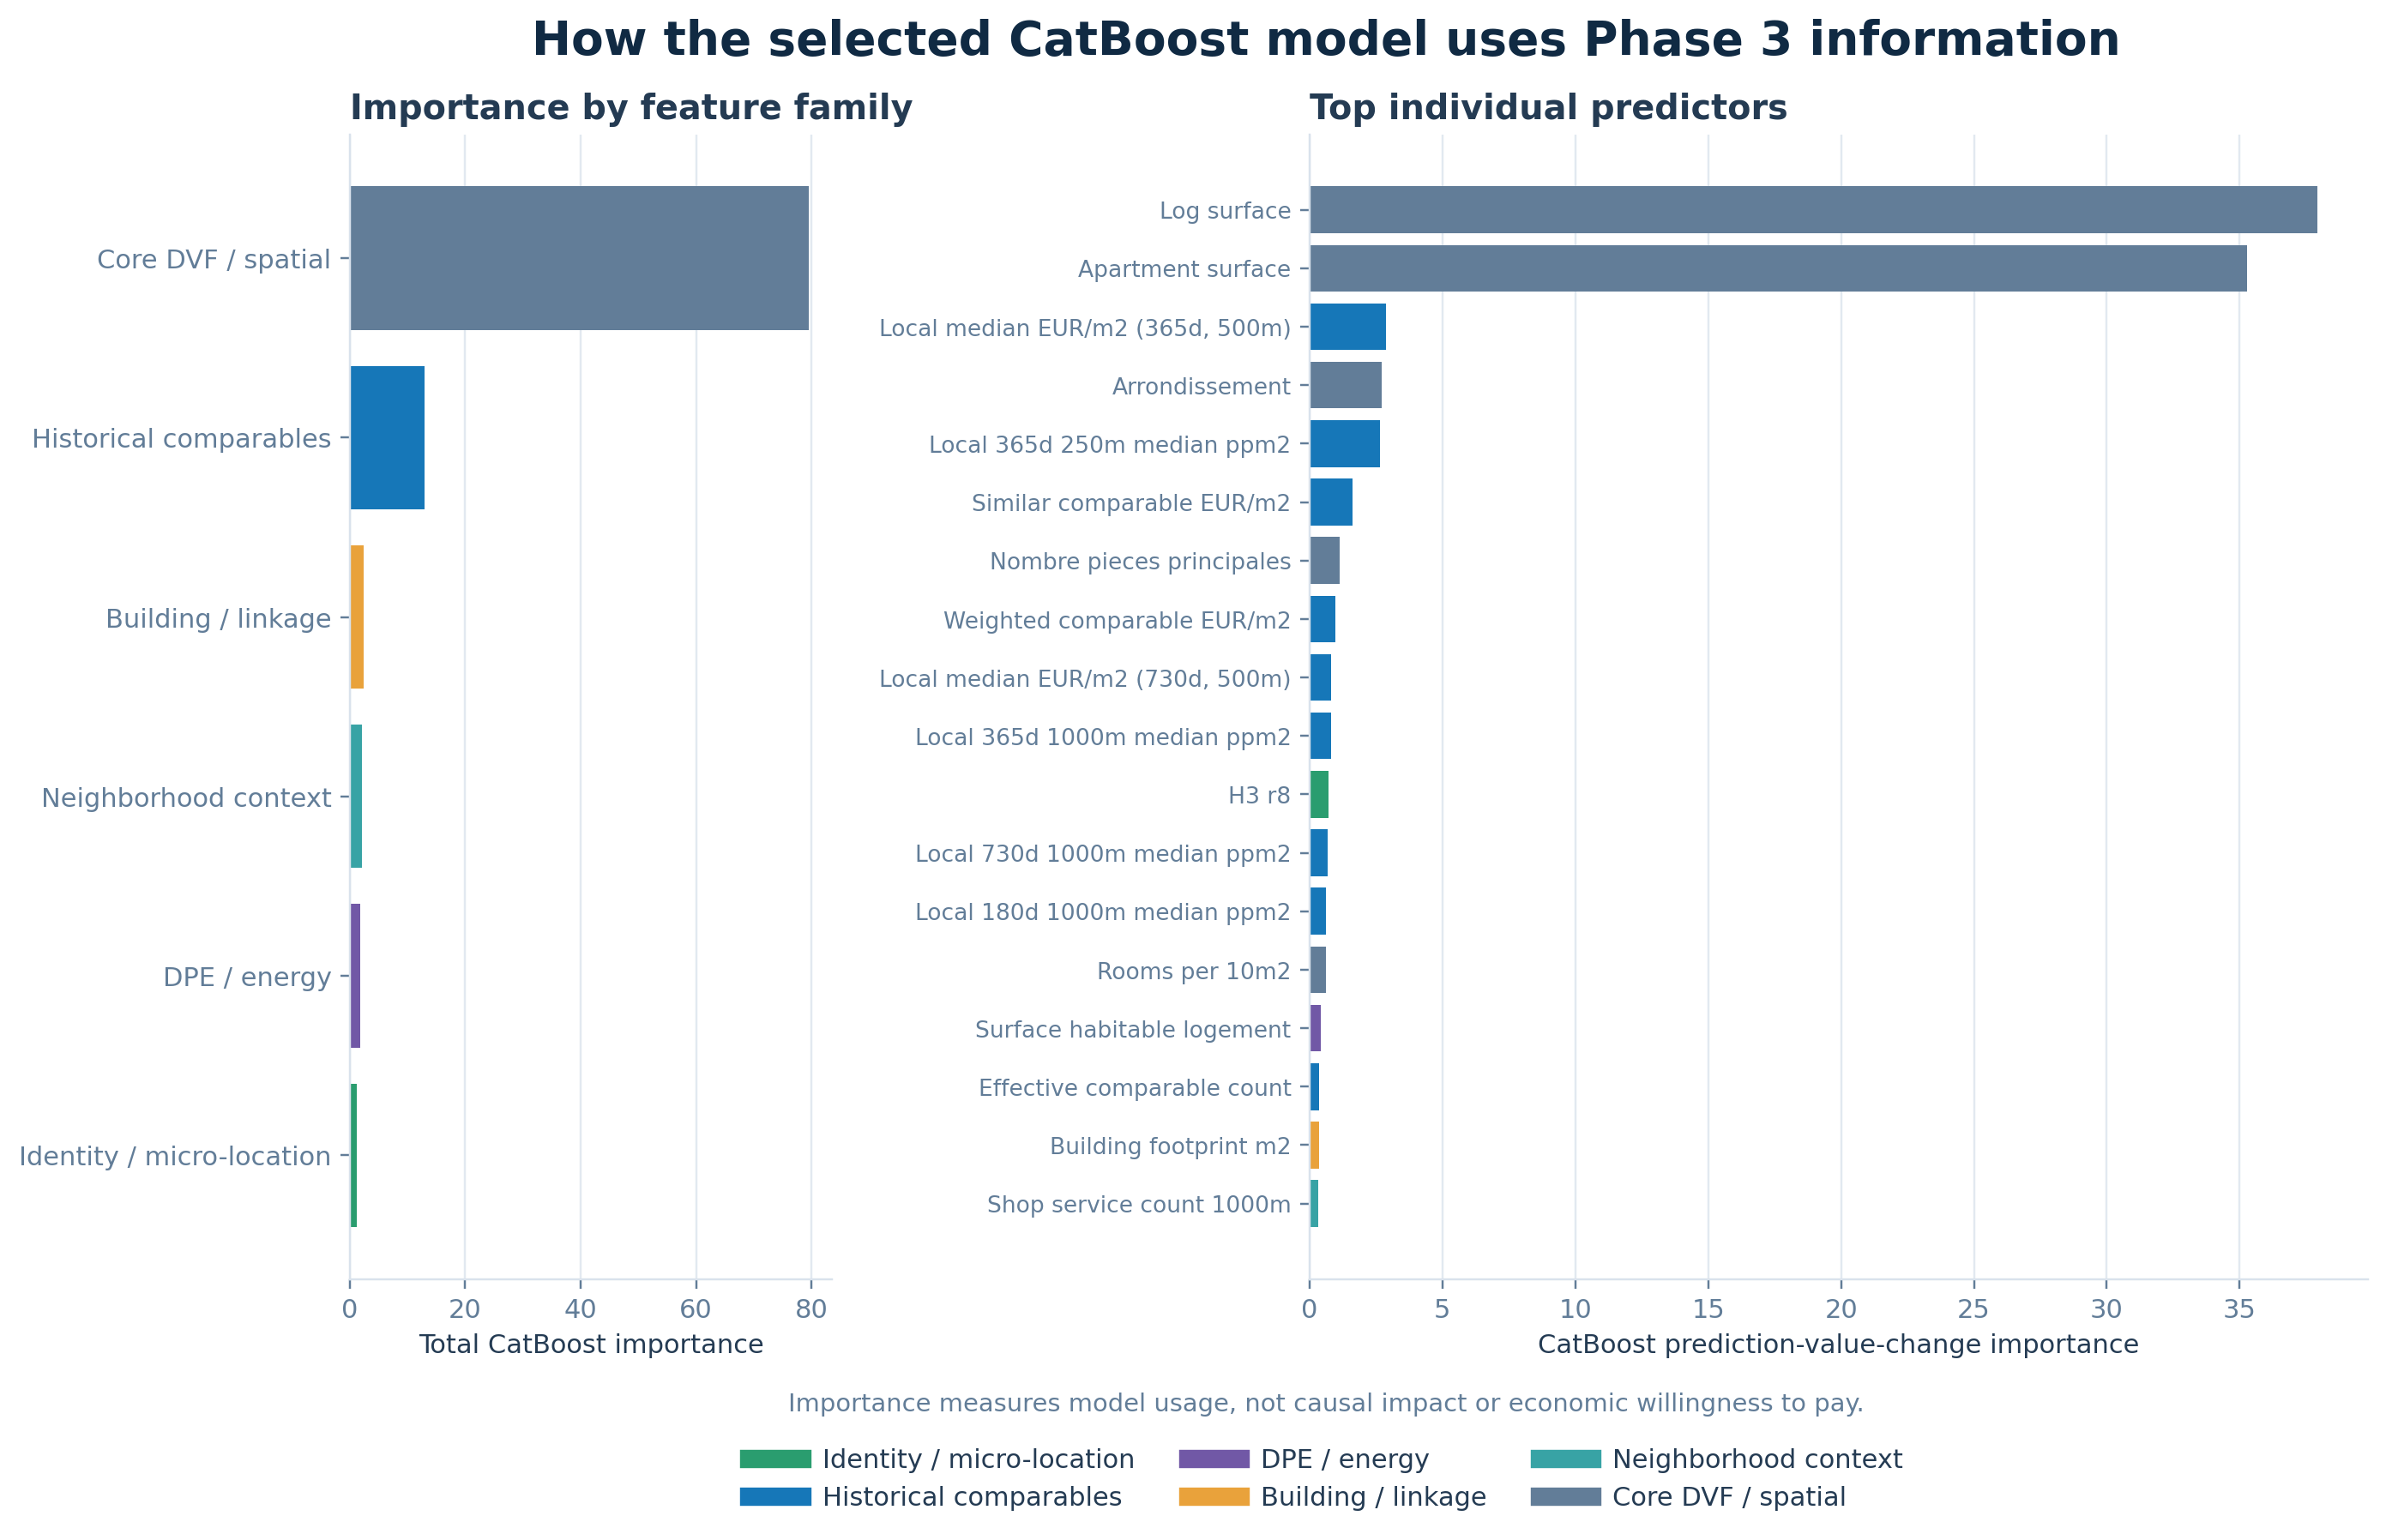
\includegraphics[width=\textwidth]{phase3_feature_importance.png}
\caption{Selected CatBoost importance by feature family and leading individual
variables.}
\label{fig:importance}
\end{figure}

\begin{figure}[H]
\centering
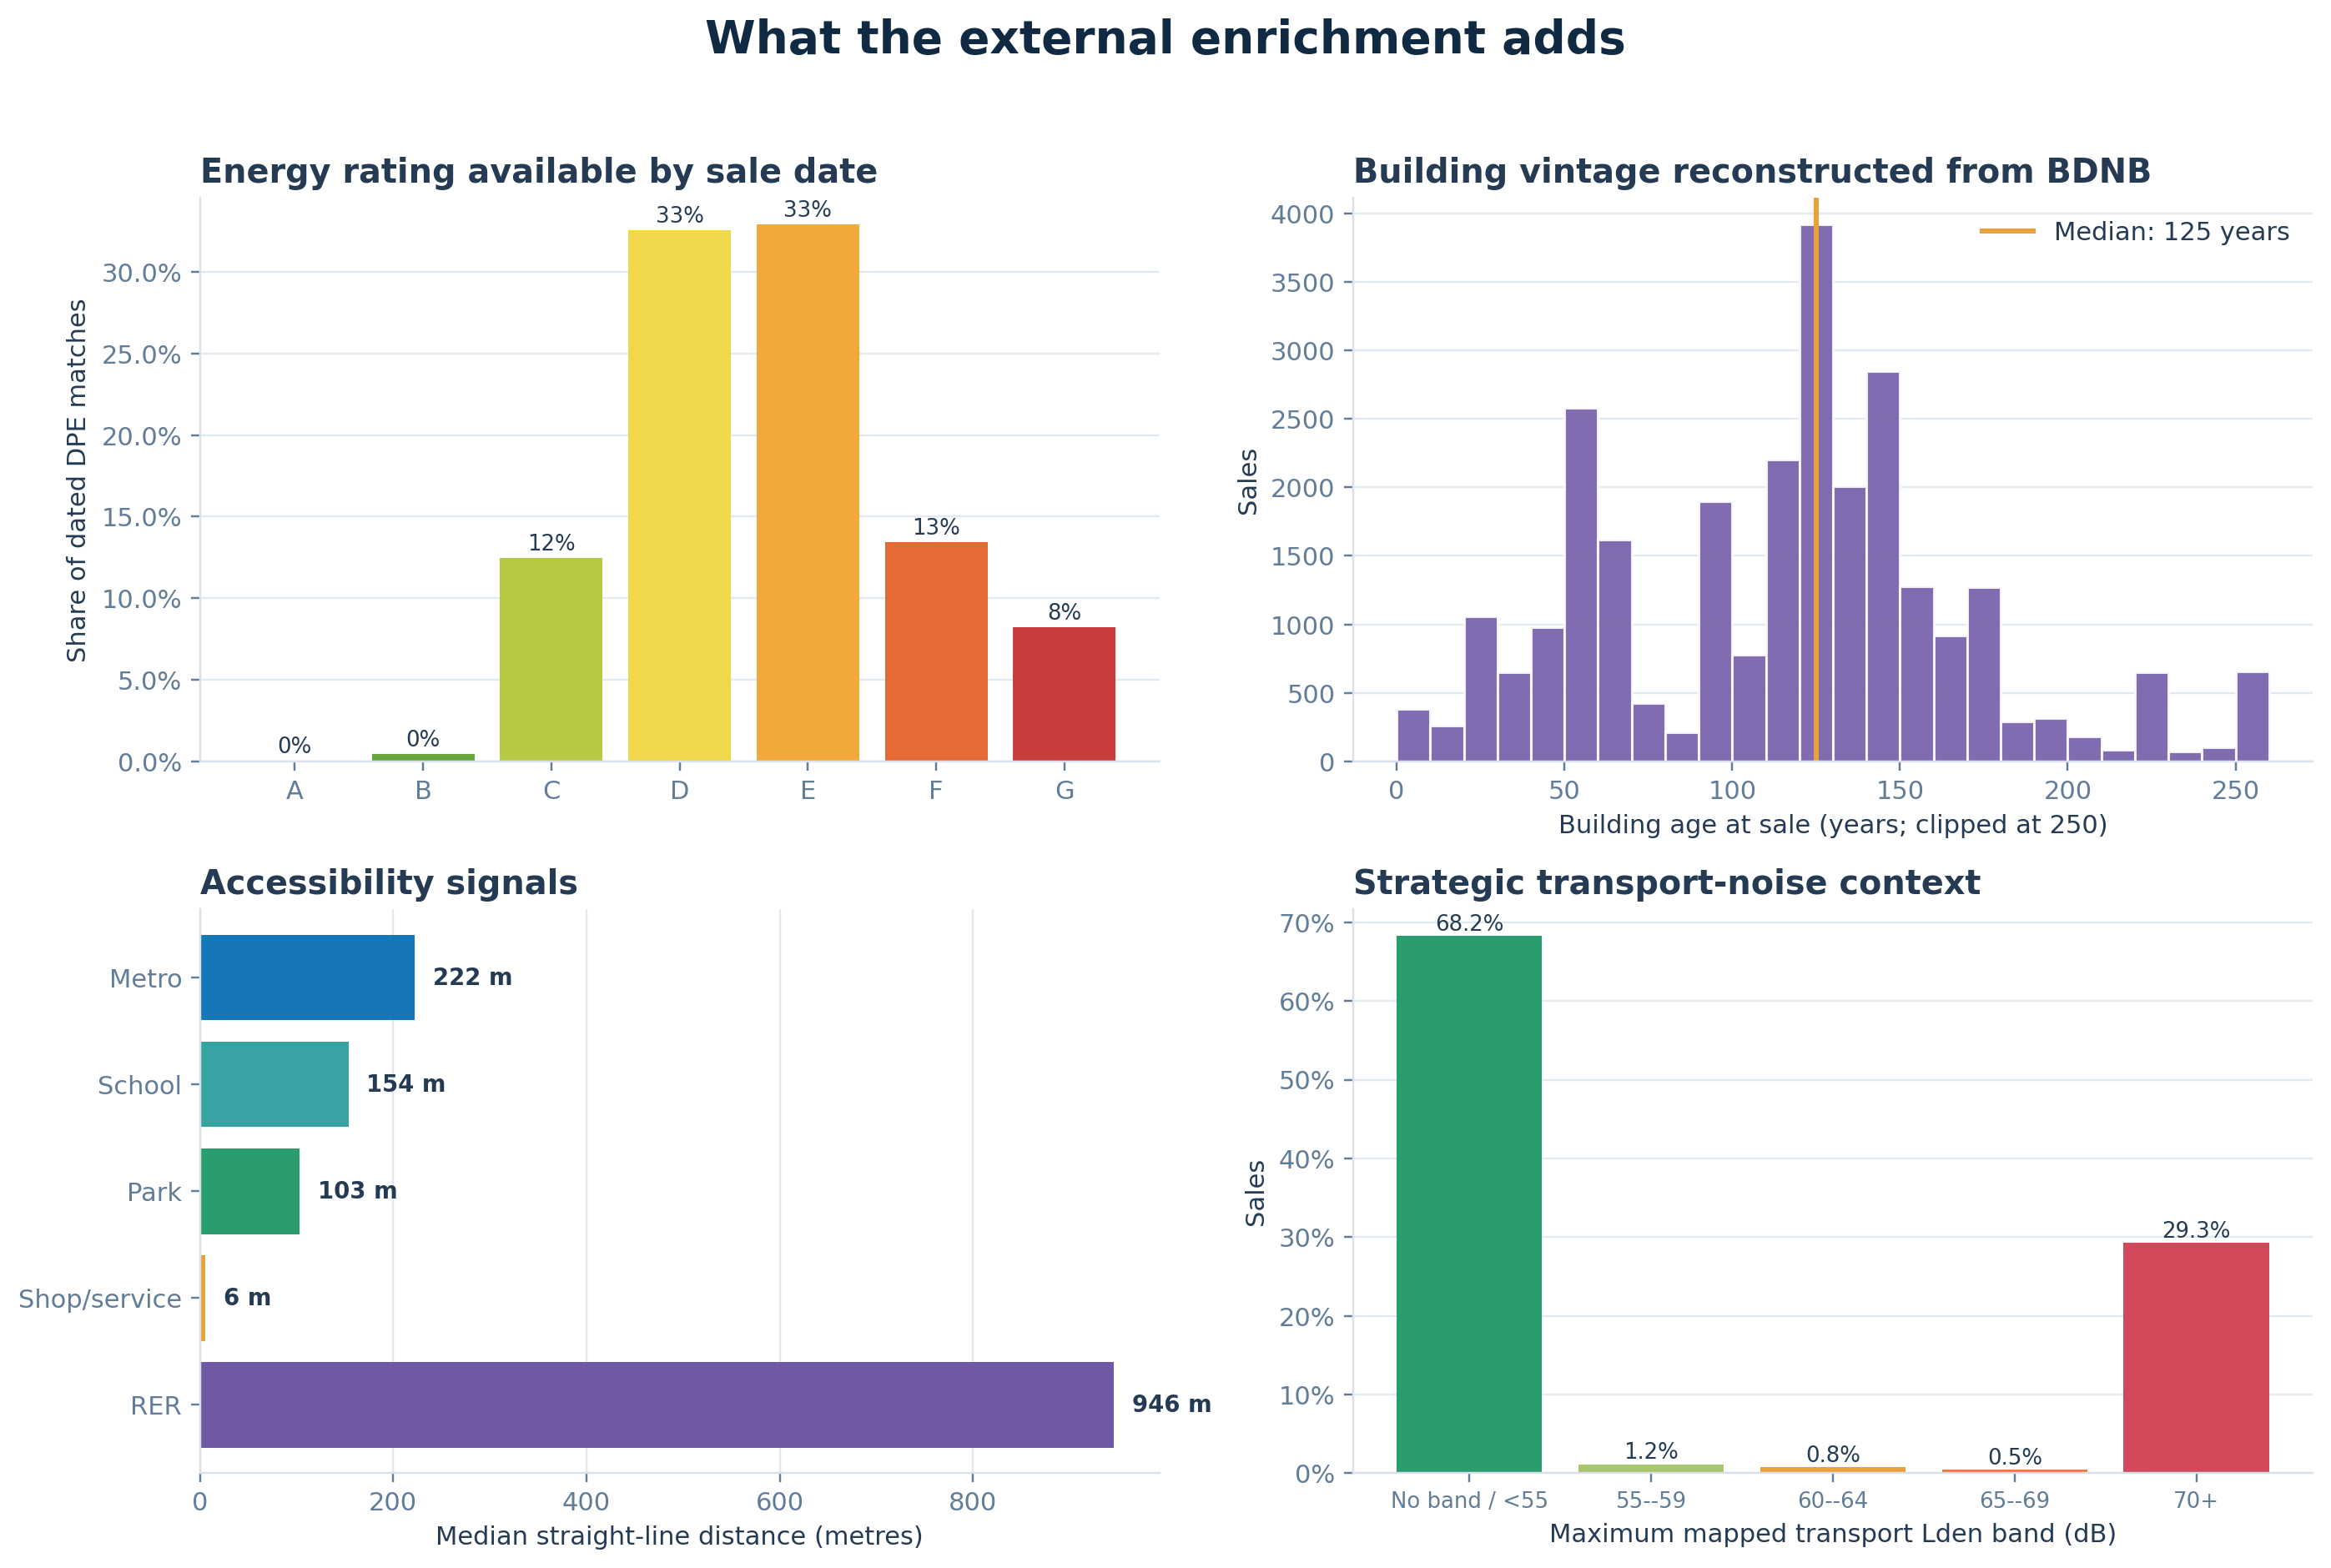
\includegraphics[width=\textwidth]{phase3_enrichment_profile.png}
\caption{Coverage and distributions of the building, energy, transport,
amenity and noise enrichment layer.}
\label{fig:enrichment}
\end{figure}

\section{Limitations and model-risk controls}

\begin{enumerate}[leftmargin=1.8em]
  \item \textbf{Retrospective-static bias.} Current BAN/BDNB and amenity
  snapshots can improve reconstruction without proving that every field was
  known historically.
  \item \textbf{Test-year familiarity.} The 2025 cohort is excluded from
  fitting and selection, but earlier project phases exposed aggregate 2025
  scores. A later untouched cohort is needed for prospective confirmation.
  \item \textbf{Missing apartment-level attributes.} Floor, elevator, interior
  condition, view, orientation, renovation and occupancy are unavailable.
  \item \textbf{DPE linkage ambiguity.} A building can contain multiple
  apartments and eligible diagnostics. Confidence and surface-difference
  fields expose but cannot remove this ambiguity.
  \item \textbf{Spatial semantics.} Straight-line distance ignores walking
  networks, barriers, station entrances and service quality.
  \item \textbf{Market-regime uncertainty.} Transaction-level bootstrap
  intervals do not capture interest-rate, regulation, tax or liquidity regime
  shifts.
  \item \textbf{Tail calibration.} The model compresses price extremes and
  should be monitored separately for luxury and very small/low-value units.
  \item \textbf{Use limitation.} Output is an automated indication with
  statistical uncertainty, not a certified appraisal or lending decision.
\end{enumerate}

\section{Recommended production roadmap}

\begin{enumerate}[leftmargin=1.8em]
  \item Freeze this benchmark and preserve its source/output checksums.
  \item Validate prospectively on the next complete DVF period without
  changing configuration after observing its labels.
  \item Add validation-fitted calibration for price tails and publish interval
  coverage by arrondissement, surface and value band.
  \item Acquire legally reusable apartment-floor, elevator and condition data;
  introduce each family through a dated ablation.
  \item Monitor monthly MAE, MdAPE, bias, within-20\% rate, missingness, match
  confidence and distribution drift.
  \item Provide a fallback to the transparent Phase 2 correction when external
  resolution or data freshness fails.
  \item Record model cards, data lineage, intended use, exclusions and human
  review requirements before deployment.
\end{enumerate}

\section{Reproducibility package}

The complete workflow is reproducible from the project root:
\begin{verbatim}
$env:PYTHONPATH = '.\src'
python -m paris_avm.features.preprocessing
python -m paris_avm.modeling.benchmark_phase2
python -m paris_avm.modeling.benchmark_phase3
python -m paris_avm.visualization.phase2
python -m paris_avm.visualization.phase3
python -m paris_avm.visualization.model_evaluation
powershell -ExecutionPolicy Bypass -File `
  .\docs\paper\compile_model_evaluation.ps1
\end{verbatim}

Primary machine-readable deliverables are:
\begin{itemize}[leftmargin=1.5em]
  \item \path{reports/preprocessing/run_summary.json};
  \item \path{reports/phase2/phase2_model_comparison.csv};
  \item \path{reports/phase3/phase3_model_comparison.csv};
  \item \path{reports/phase3/phase3_test_predictions.csv};
  \item \path{reports/model_evaluation/segment_performance.csv};
  \item \path{reports/model_evaluation/calibration_by_value_decile.csv};
  \item \path{reports/model_evaluation/feature_importance.csv}; and
  \item \path{reports/model_evaluation/feature_family_importance.csv}.
\end{itemize}

\section{Conclusion}

The five proposed preprocessing layers are fully implemented, tested and run
on the complete Paris cohort. The data contract is explicit, row identity is
preserved, target leakage is controlled for current-sale price and dated DPE,
and chronological evaluation is enforced. Retraining confirms that external
building, energy and neighborhood enrichment produces a real but bounded
improvement over a strong comparable-sale reference. The selected 100-input
CatBoost model reduces 2025 MAE by EUR 3,231, improves every month and
arrondissement, and preserves strong overall $R^2$. Its remaining weaknesses
are concentrated in price extremes and missing apartment-level condition.

The professional conclusion is therefore balanced: the enriched model is the
best research benchmark and a credible AVM component, while prospective
validation, temporal source vintages, tail calibration and human appraisal
controls remain necessary before high-stakes use.

\appendix
\section{Feature-contract inventory}

\begin{longtable}{p{3.4cm}p{12.2cm}}
\caption{Model-input inventory by family.}\label{tab:features}\\
\toprule
Family & Inputs \\
\midrule
\endfirsthead
\toprule
Family & Inputs \\
\midrule
\endhead
Property & \texttt{surface\_reelle\_bati}, \texttt{nombre\_pieces\_principales},
\texttt{adresse\_numero}, \texttt{nombre\_lots}, \texttt{log\_surface},
\texttt{rooms\_per\_10m2}, \texttt{surface\_terrain} \\
Time & \texttt{month}, \texttt{day\_of\_year}, \texttt{year},
\texttt{months\_since\_2021} \\
Coordinates and spatial & \texttt{latitude}, \texttt{longitude},
\texttt{x\_l93}, \texttt{y\_l93}, \texttt{distance\_paris\_center\_m},
\texttt{bearing\_sin}, \texttt{bearing\_cos}, \texttt{h3\_r8},
\texttt{h3\_r9}, \texttt{code\_postal} \\
Historical comparables & Seven local count/median pairs; 365-day/500-m MAD;
weighted and similar-weighted price per m$^2$; similar/effective counts;
nearest prior distance; median comparable age; 180-versus-365-day momentum at
500 m and 1,000 m \\
Building/linkage & BAN distance/confidence; BDNB confidence and candidate counts;
levels, year, dwelling count, height, footprint, parking/total lots, age,
year-missing flag, use, wall/roof materials, state and RNC period \\
DPE/energy & availability, age, surface difference, confidence, construction
year, dwelling/building levels and surfaces, energy consumption, GHG emissions,
DPE/GHG classes, heating installation and heating energy \\
Neighborhood context & metro/RER/train/tram distance; station-mode and line
counts; school distance/count; green-space distance/count/area; service
distance/counts; road, RATP, SNCF and maximum transport noise \\
External identity & \texttt{ban\_address\_id}, \texttt{bdnb\_building\_id},
\texttt{bdnb\_match\_method} \\
\bottomrule
\end{longtable}

\section{Machine-readable diagnostic tables}

The PDF intentionally reports interpretable aggregates rather than every CSV
row. Complete results for 12 months, 20 arrondissements, six surface bands, six
value bands, comparable-density bands, DPE availability and ten calibration
deciles are stored in \path{reports/model_evaluation/segment_performance.csv}
and \path{reports/model_evaluation/calibration_by_value_decile.csv}. These
tables are generated directly from the frozen prediction export and are the
source of Figures~\ref{fig:segments} and~\ref{fig:coveragecalibration}.

\begin{thebibliography}{9}
\bibitem{dvf}
Direction g\'en\'erale des Finances publiques.
\emph{Demandes de valeurs fonci\`eres (DVF)}.
\url{https://www.data.gouv.fr/fr/datasets/demandes-de-valeurs-foncieres/}.

\bibitem{ban}
Institut national de l'information g\'eographique et foresti\`ere.
\emph{Base Adresse Nationale}.
\url{https://adresse.data.gouv.fr/}.

\bibitem{bdnb}
Centre scientifique et technique du b\^atiment.
\emph{Base de Donn\'ees Nationale des B\^atiments}.
\url{https://www.data.gouv.fr/fr/datasets/base-de-donnees-nationale-des-batiments/}.

\bibitem{dpe}
ADEME. \emph{Diagnostics de performance \'energ\'etique pour les logements}.
\url{https://data.ademe.fr/}.

\bibitem{catboost}
L. Prokhorenkova et al. CatBoost: unbiased boosting with categorical features.
\emph{Advances in Neural Information Processing Systems}, 31, 2018.

\bibitem{lightgbm}
G. Ke et al. LightGBM: a highly efficient gradient boosting decision tree.
\emph{Advances in Neural Information Processing Systems}, 30, 2017.
\end{thebibliography}

\end{document}
